\documentclass[a4paper,11pt]{report}
\usepackage[utf8]{inputenc}
\usepackage[T1]{fontenc}
\usepackage[english,main=french]{babel}
\usepackage[babel=true]{csquotes}
\usepackage{translator}
\usepackage{graphicx}
\usepackage{float}
\usepackage[export]{adjustbox}
\usepackage{amsmath}
\usepackage{amsfonts}
\usepackage{algorithm2e}
\usepackage{hyperref}
\usepackage{listings}
\usepackage{pgfgantt}
\usepackage[toc,page]{appendix}
\usepackage[backend=biber,style=alphabetic]{biblatex}
\usepackage{glossaries}
\usepackage[top=2.5cm,bottom=2.5cm,left=3cm,right=3cm]{geometry}
\usepackage{tikz}
\usepackage{microtype}

\providetranslation[to=french]{April}{Avril}
\providetranslation[to=french]{May}{Mai}
\providetranslation[to=french]{June}{Juin}
\providetranslation[to=french]{July}{Juillet}
\providetranslation[to=french]{August}{Août}

\graphicspath{ {../images/} }
\bibliography{refs.bib}
\nocite{*}
\RestyleAlgo{ruled}
\renewcommand{\appendixpagename}{Annexes}
\renewcommand{\appendixtocname}{Annexes}
\hypersetup{
    colorlinks=true, %colorise les liens
    breaklinks=true, %permet le retour  la ligne dans les liens trop longs
    urlcolor=blue, %couleur des hyperliens
    linkcolor=black, %couleur des liens internes
    bookmarksopen=true, %si les signets Acrobat sont crs, les afficher compltement.
}
\lstset{
    basicstyle=\ttfamily,
    breaklines=true,
    showstringspaces=false,
    keywordstyle=\color{blue},
    commentstyle=\color{red}
}
\usetikzlibrary{arrows,positioning}
\usetikzlibrary{calc}


\title{Rapport de stage}
\author{Oscar Buon}


\begin{document}


\begin{titlepage}
    \centering
    \begin{minipage}{0.25\textwidth}
        
\includegraphics[width=\textwidth]{logo_ISIMA_INP.png}
    \end{minipage}\hfill
    \begin{minipage}{0.25\textwidth}
        
\includegraphics[width=\textwidth]{logo_CERN.png}
    \end{minipage}\hfill
    \begin{minipage}{0.25\textwidth}
        
\includegraphics[width=\textwidth]{logo_LHCb.png}
    \end{minipage}

    \vfill

    {\Large
        Rapport d'élève ingénieur \par
        Stage de 2ème année \par
        Filière 1 : Informatique des systèmes interactifs pour l’embarqué, la robotique et le virtuel \par
    }

    \vfill

    {\huge\bfseries Speeding up LHCb software through compilation optimization \par}

    \vfill

    {\Large Présenté par : Oscar Buon \par}

    \vfill

    \begin{minipage}{0.65\textwidth}
        \textsc{Responsable ISIMA : Mamadou Kanté}\\
        \textsc{Responsable Entreprise : Sébastien Ponce}\\
    \end{minipage}
    \hfill
    \begin{minipage}{0.25\textwidth}
        \textsc{4 septembre 2023} \\
        \textsc{Stage de 5 mois} \\
    \end{minipage}

    \vfill

    Campus des Cézeaux. 1 rue de la Chebarde. TSA60125. 63178 Aubière CEDEX
\end{titlepage}


\pagenumbering{Roman}
\chapter*{Remerciements}
J'aimerais commencer par remercier Sébastien Ponce, mon tuteur de stage sans qui mon travail au CERN n'aurait pas été possible et qui m'a aidé tout au long.

Merci également à M. Mamadou Kanté, tuteur ISIMA et responsable de la filière.

\bigskip
Je tiens aussi à remercier Alexandre Boyer qui m'a permis à l'occasion du forum ingénieur de trouver un stage au CERN.

\bigskip
Merci à Marco Clemencic qui m'a plusieurs fois aidé à résoudre certains problèmes.

\bigskip
Enfin je remercie Gloria Corti et Marco Cattaneo qui m'ont fait visité LHCb et DELPHI sous terre.

\tableofcontents

\listoffigures


\begin{abstract}

    Ce stage a pour objectif d'étudier l'infrastructure logicielle qui traite les données du détecteur LHCb du CERN et de mettre en place des solutions pour optimiser ses performances via une meilleure compilation.
    Les programmes sont principalement codés en C++ et compilés via CMake.

    Plusieurs méthodes ont été utilisées.
    La première a consisté à fusionner les centaines de bibliothèques dynamiques en un seul exécutable statique.
    L'utilisation de profile-guided optimization et de link-time optimization a ensuite été mise en place.
    Enfin les options \emph{fast-math} ont été testées.

    Au total, une amélioration de la vitesse d'exécution d'environ $11\%$ a été obtenue avec le link-time optimization, le profile-guided optimization et fast-math sur le code de la reconstruction des données du détecteur.

    Le reste du temps a été utilisé pour mettre en place l'outil include-what-you-use et la compilation sur ARM.
    \vfill

    Mots-clés : LHCb, Optimisation, Compilation avancée

\end{abstract}

\begin{otherlanguage}{english}
    \begin{abstract}

        \vfill

        Keywords : LHCb, Optimization, Advanced compilation
    \end{abstract}
\end{otherlanguage}


\pagenumbering{arabic}
\chapter*{Introduction}
LHCb est l'une des quatre expériences principales du Large Hadron Collider (LHC) du CERN.
Au centre du détecteur ont lieu plus de 30 millions de collisions par secondes, ce qui produit un flux de données d'environ $5 To/s$.
Ces données doivent rapidement être traitées pour reconstruire les trajectoires des particules et pour pouvoir être analysées dans le monde entier.

L'infrastructure logicielle de traitement est principalement écrite en C++ et en Python.
Du code est ajouté ou modifié tous les jours par plusieurs centaines de membres de la collaboration, qui représentent 83 instituts dans 19 pays en 2020.
Cela représente des millions de lignes de codes qu'il faut maintenir et améliorer.
Pour gérer cela, des outils modernes comme Git \cite{git}, gcc \cite{gcc}, clang \cite{clang} ou CMake \cite{cmake} sont utilisés.

L'objectif du stage est d'abord de proposer puis d'implémenter des solutions pour améliorer l'efficacité des programmes en jouant sur la compilation.
Le temps restant est consacré à effectuer d'autres tâches aidant au maintient de l'infrastructure.

Dans un premier temps a été étudié la possibilité d'utiliser des \emph{bibliothèques statiques} (\ref{section:static}) à la place des \emph{dynamiques}.
Ensuite a été abordé la mise en place de \emph{profile-guided optimization} (\ref{section:pgo}) pour la compilation des programmes.
Aussi l'impact de l'utilisation de \emph{fast math} (\ref{section:fast-math}) sur la rapidité et la stabilité des programmes a été étudié.
La mise en place de l'outil \emph{incude-what-you-use} (\ref{section:iwyu}) permettant de mieux gérer les inclusions dans le code source a été envisagée.
Enfin, la compilation de la pile LHCb pour architecture \emph{ARM} (\ref{section:arm}) a été étudiée.

La première partie de ce rapport est consacrée à l'étude et l'analyse des problèmes.
La seconde explique les méthodes et solutions techniques utilisées.
La dernière rend compte des résultats.


\chapter{Introduction du travail à faire}
\section{Présentation du CERN}
L'Organisation européenne pour la recherche nucléaire (\href{https://home.cern/}{CERN}) est le plus grand laboratoire d'étude de la physique des particules au monde.
Le centre, qui a été fondé en 1954, se situe sur la frontière franco-suisse à quelques kilomètres de Genève, le site principal étant à Meyrin.

Les recherches effectuées au CERN utilisent différents accélérateurs de particules.
Le principe est de faire atteindre à des particules des vitesses proches de celle de la lumière pour qu'elles acquièrent une grande énergie cinétique, puis de les faire entrer en collision.
La physique des particules prévoit alors la création de nouvelles particules selon l'équation $E=mc^2$ où l'énergie peut être transformée en masse.
Ainsi en détectant les particules résultantes de ces collisions et en comparant avec les théories existantes, on peut les valider ou les invalider.

Il existe plusieurs accélérateurs et un grand nombre d'expériences au CERN.
Le plus grand accélérateur est le Grand collisionneur de hadrons ou LHC pour Large Hadron Collider (Figure \ref{LHC}), qui a été mis en fonction en 2008 et qui a une circonférence d'environ 27 kilomètres.
Il permet d'accélérer des protons à une énergie d'environ $7 Tev$.

\begin{figure}[!htb]
    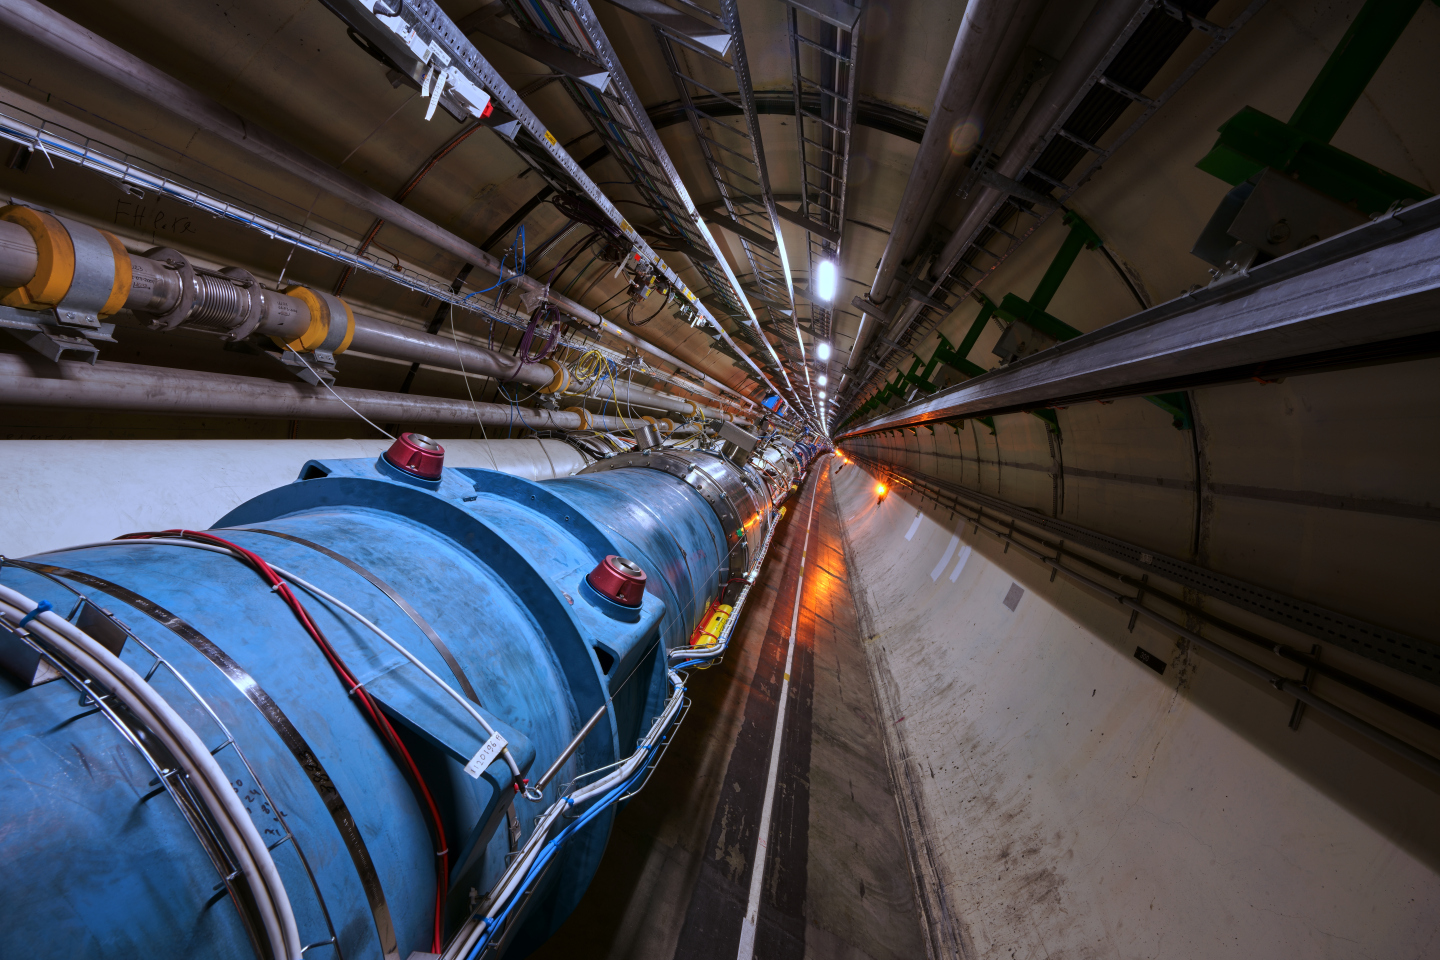
\includegraphics[width=0.75\textwidth, center]{LHC.jpg}
    \caption{Tunnel du LHC}
    \label{LHC}
\end{figure}

Le CERN est connu pour être à l'origine de plusieurs découvertes importantes.
On peut notamment citer la découverte du boson de Higgs en 2012 qui a mené au prix Nobel de François Englert et Peter Higgs.
Le CERN est aussi à l'origine de la création du World Wide Web (Figure \ref{WEB}), qui permettait à l'origine le partage d'articles scientifiques.

\begin{figure}[!htb]
    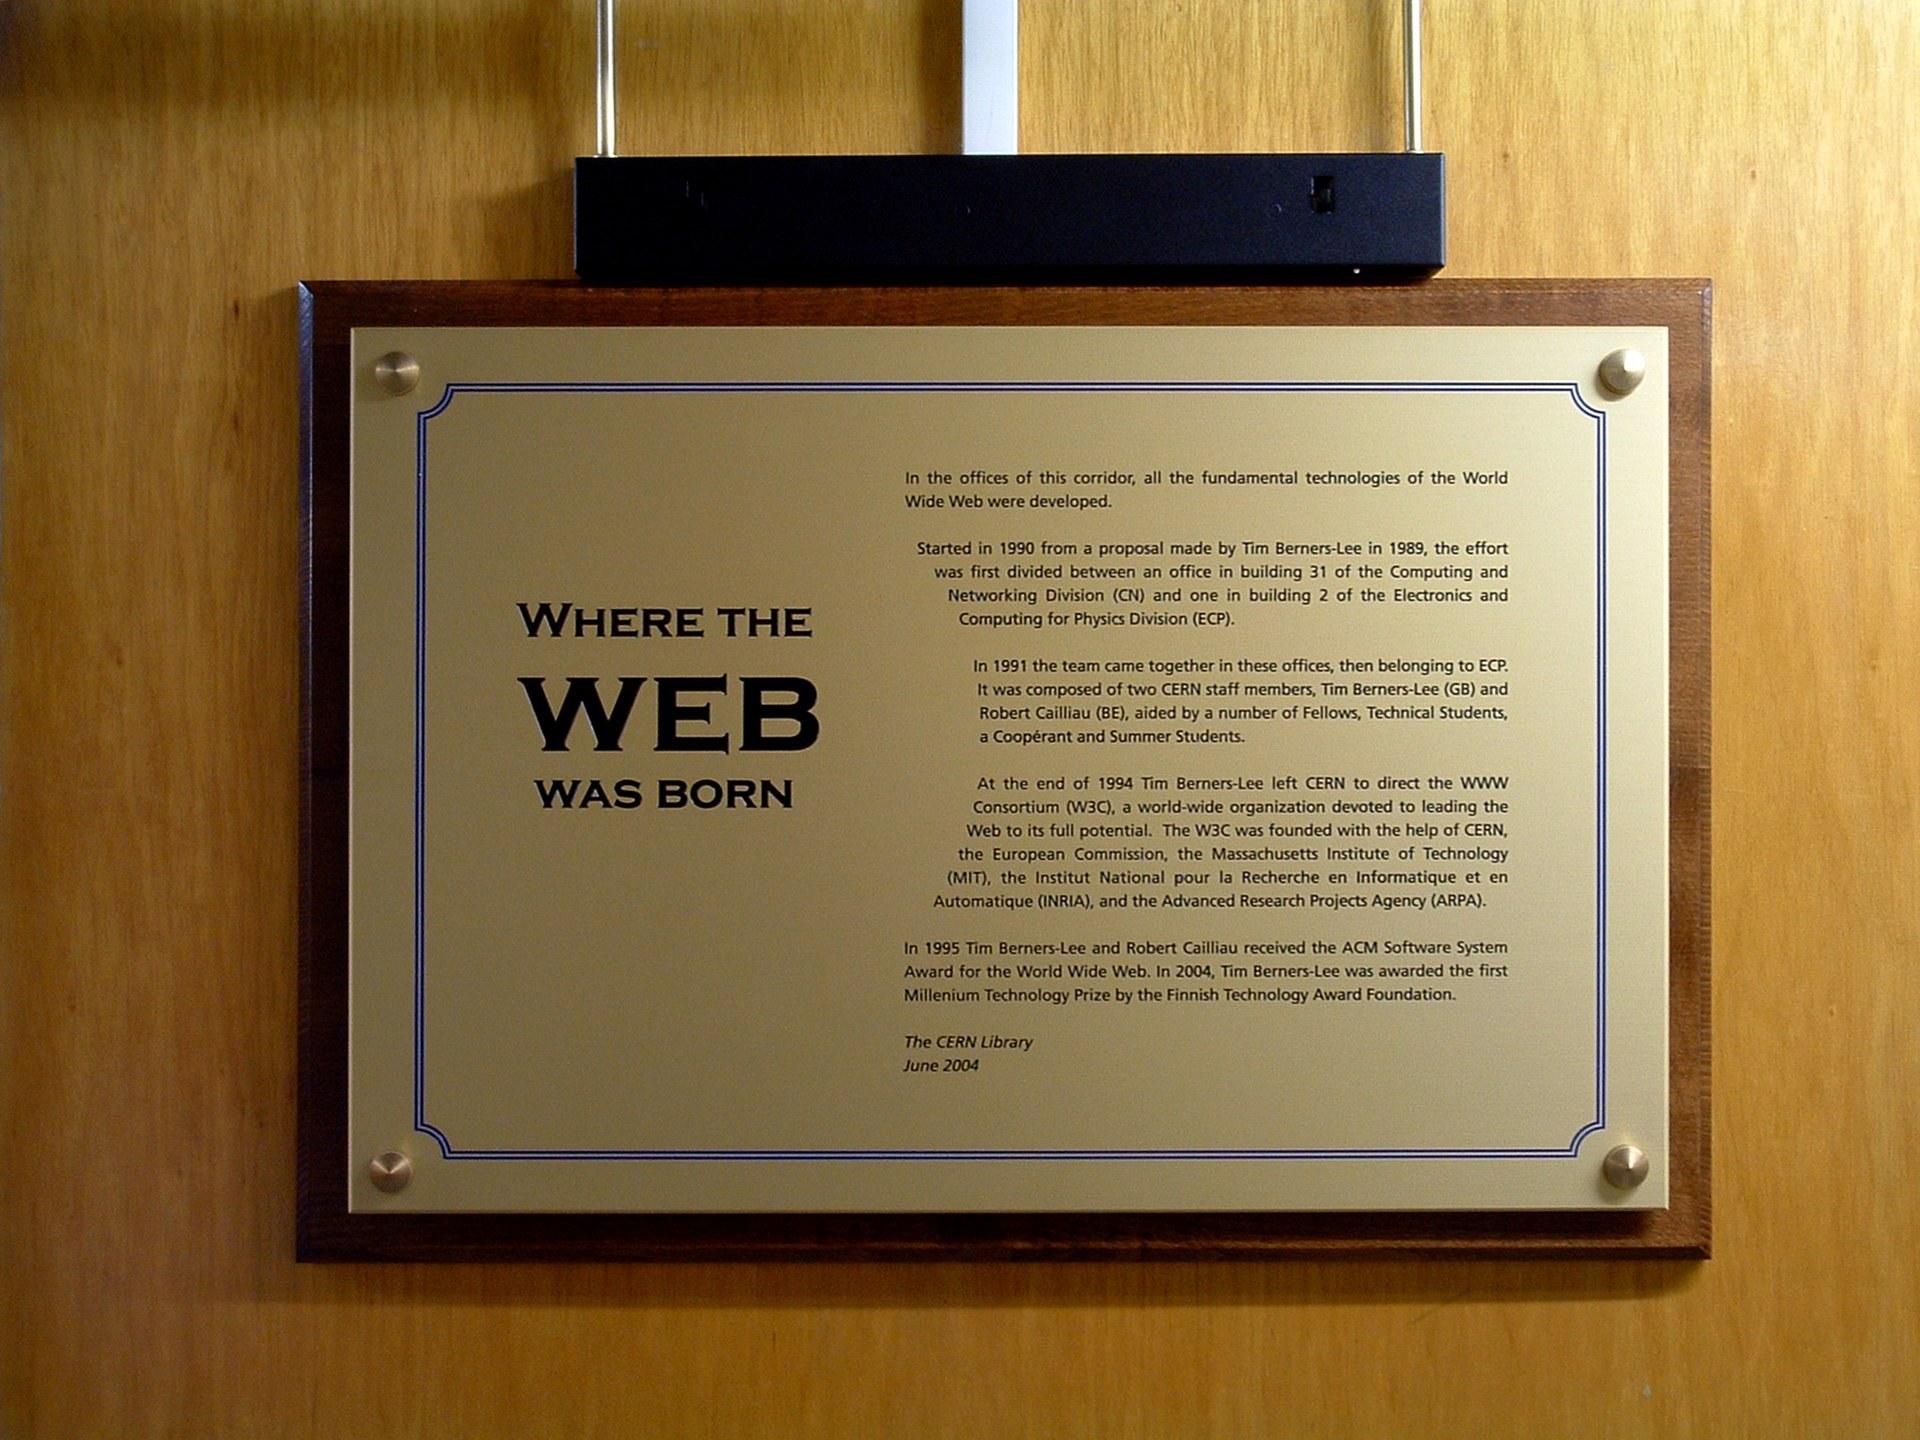
\includegraphics[width=0.75\textwidth, center]{WEB.jpg}
    \caption{Plaque commémorative de l'invention du World Wide Web dans le bâtiment 1 du CERN}
    \label{WEB}
\end{figure}

Sur le LHC sont installés quatre principales expériences qui sont des collaborations internationales : ATLAS, CMS, ALICE et LHCb.
Ces expériences prennent la forme de détecteurs. C'est en leurs centres que se font les collisions dont les résidus sont détectés par plusieurs types de capteurs.

La mise en oeuvre des détecteurs et expériences du CERN a depuis longtemps nécessité le développement de nouvelles technologies.
Ainsi l'informatique et internet sont présent depuis longtemps afin de gérer la masse de données produites dans les détecteurs \cite{Saikumar:2022mgb}.
Des programmes comportant plusieurs millions de lignes de codes sont exécutées dans les centres de calcul sur les sites du CERN
mais aussi partout autour du monde grâce au "\href{https://wlcg-public.web.cern.ch/}{Grid}", une interconnexion de centaines de centres de calculs.
Le CERN a aussi contribué au développement d'internet en Europe.

\section{L'expérience LHCb}
Le Large Hadron Collider beauty ou \href{https://lhcb.web.cern.ch/}{LHCb} (Figure \ref{LHCb}) est l'une des quatre grandes expériences installées sur le LHC.
Elle utilise l'étude du quark b afin de mesurer l'asymétrie entre matière et antimatière.
La collaboration regroupe plus de 1200 personnes représentant plusieurs dizaines d'instituts.
L'expérience est située sur le point 8 du LHC, sur la commune française de Ferney-Voltaire.

\begin{figure}[!htb]
    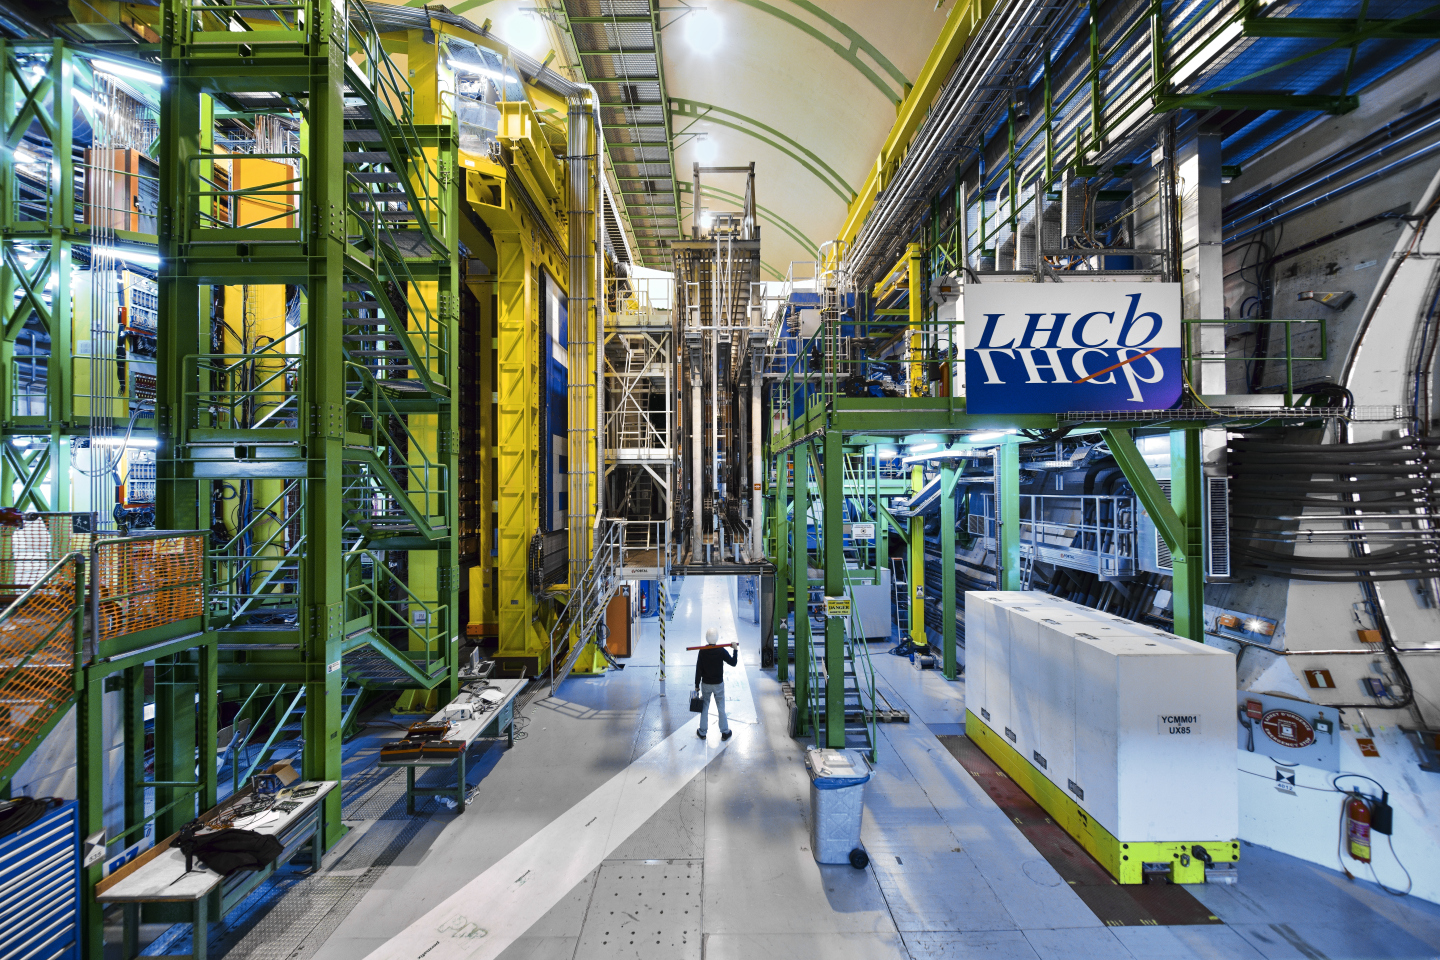
\includegraphics[width=0.75\textwidth, center]{LHCb.jpg}
    \caption{LHCb}
    \label{LHCb}
\end{figure}

Le détecteur est composé de plusieurs instruments qui mesurent le passage des particules émises lors des collisions.
Grâce aux données recueillies, on peut reconstruire les trajectoires des particules ainsi que certaines de leur propriétés comme la masse, la charge ou l'énergie (Figure \ref{LHCb_3D}).

\begin{figure}[H]
    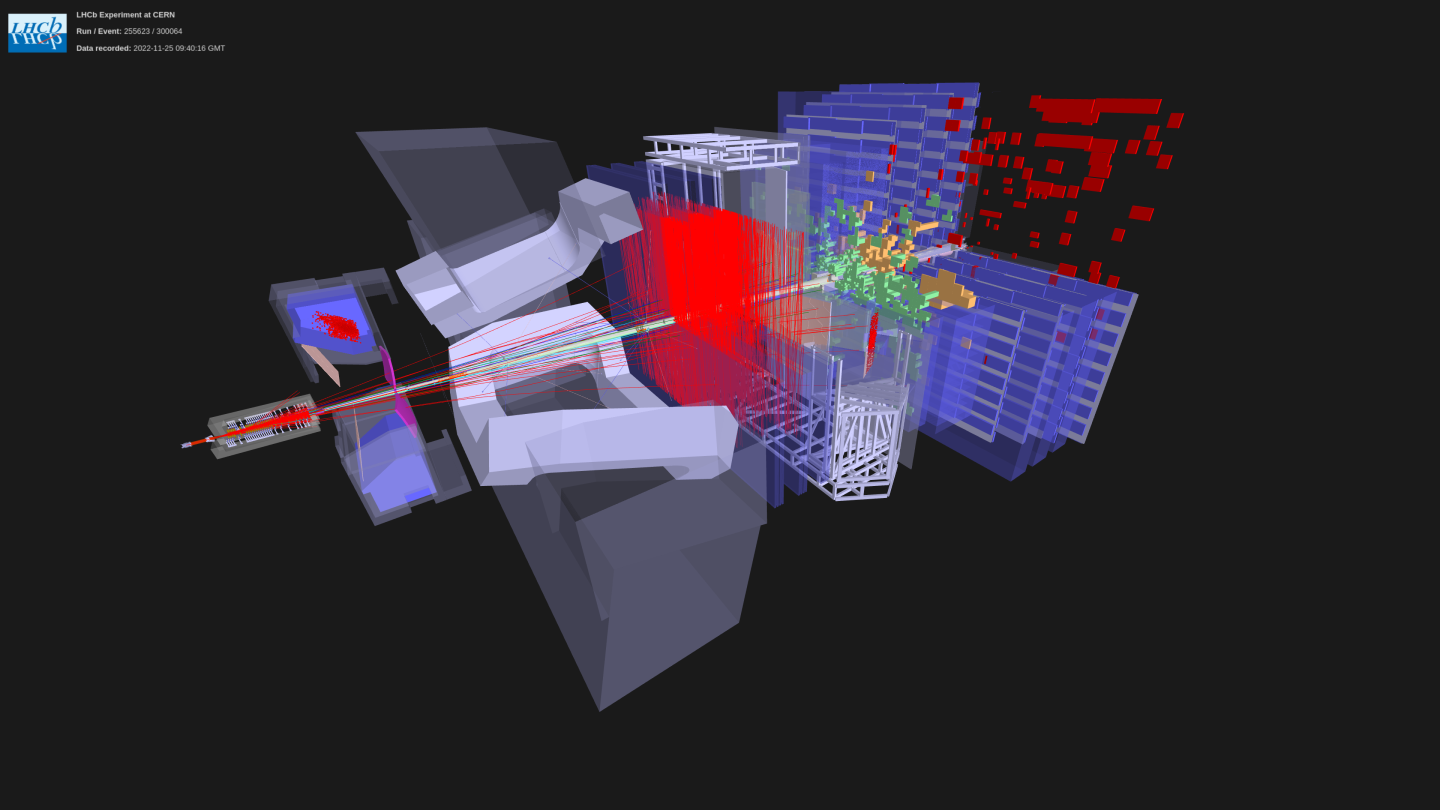
\includegraphics[width=\textwidth, center]{LHCb_3D.png}
    \caption{Visualisation de particules vues par le détecteur}
    \label{LHCb_3D}
\end{figure}

\section{Computing Group}
Les différents instruments du détecteur produisent un flux de données conséquent d'environ $5 To/s$.
Une importante infrastructure informatique est donc nécessaire pour pouvoir les traiter.
On voit sur la figure \ref{LHCb_stack} que les données sont d'abord partiellement traitées à un premier niveau de reconstruction partielle \emph{High Level Trigger 1} (Hlt1) qui permet de ne garder seulement les collisions les plus intéressantes.
Cela abaisse le flux de données à environ $100 Go/s$.
Les données sont ensuite enregistrées dans un \emph{buffer} pour quelques heures puis sont traitées par un second niveau de reconstruction complète \emph{High Level Trigger 2} (Hlt2), qui lui aussi ne garde que certaines collisions.
Ce qui en sort peut finalement être enregistré à long terme sur bandes magnétiques pour servir de matière à des recherches physiques plus tard.

\begin{figure}[H]
    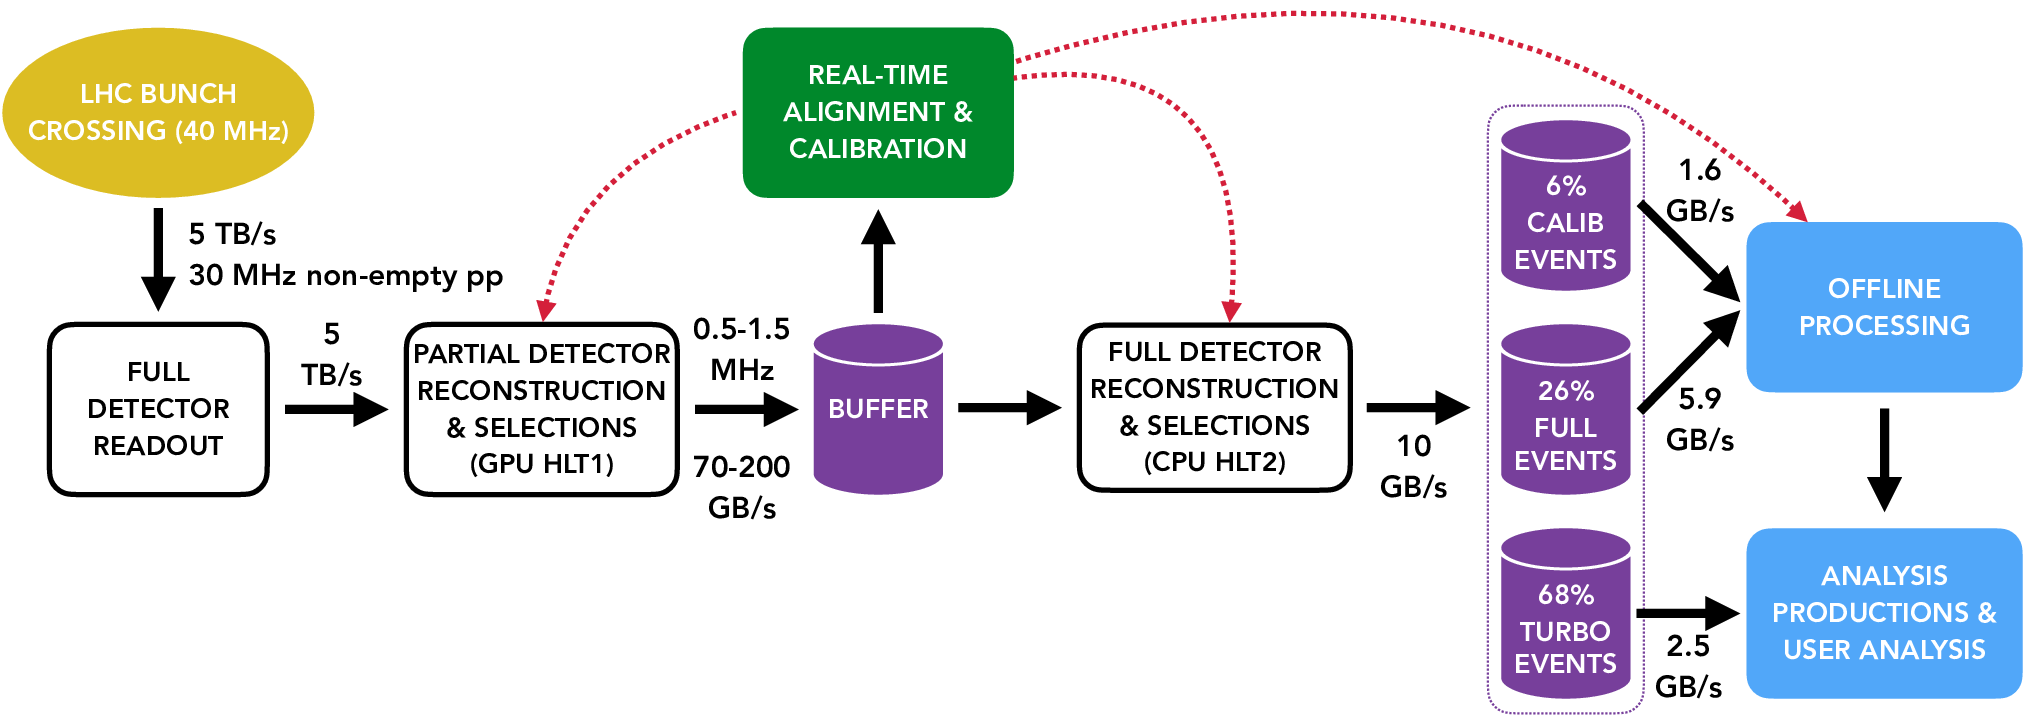
\includegraphics[width=\textwidth, center]{LHCb_stack.png}
    \caption{Infrastructure de gestion des données issues du détecteur}
    \label{LHCb_stack}
\end{figure}

LHCb utilise une pile de programmes (dont certains sont partagés avec d'autres expériences) qui traitent les données issues du détecteur.
Cette pile contient plusieurs millions de lignes de codes.
Ce code est principalement du C++ écrit en grande partie par des physiciens non ingénieurs en informatique et dont certaines parties ont plusieurs décennies d'âge.

Son maintien et son amélioration sont donc des enjeux majeurs.
C'est le Computing Group de LHCb qui est chargé de cette tâche et c'est en son sein que s'est fait le stage.

\section{Objectif du stage}
Le code C++ de LHCb est compilé avec l'outil CMake \cite{cmake} qui permet de simplement définir les différentes cibles de compilation ainsi que leurs dépendances.
Il est composé de plusieurs programmes qui forment une pile.
On peut citer : Geant, Root ou Gaudi qui sont partagés avec d'autres expériences et Detector, LHCb, Lbcom, Rec ou Moore qui sont spécifiques à LHCb.
Tout ceci tourne sur des serveurs Linux et est largement parallélisé.

L'objectif de ce stage est d'implémenter des solutions basées sur une meilleure utilisation du compilateur pour améliorer la rapidité d'exécution du code.
Les deux principales voies initialement envisagées sont l'utilisation de bibliothèques statiques à la place des dynamiques et la mise en place de profile-guided optimization.
D'autres sujets ont ensuite été traités : les options de fast-math, la mise en place d'include-what-you-use, et la compilation sur ARM.

\section{Étude et analyse des problèmes}

\subsection{Étapes de compilation}
Un programme écrit dans un langage de programmation comme le C ou le C++ ne peut pas être exécuté directement.
Il doit d'abord être transformé en un fichier binaire exécutable par le système.
On appelle ce processus la compilation.
Le passage du code source au binaire final se fait en plusieurs étapes :
\begin{enumerate}
    \item Le \emph{préprocesseur} prépare le code source en exécutant les macros et les autres directives.
          C'est notamment lui gère les inclusions entre fichiers.
    \item Le \emph{compilateur} fait l'analyse lexicale et syntaxique pour produire du code assembleur à partir du code source.
          Il peut également faire des optimisations.
          C'est l'étape la plus importante.
    \item L'\emph{assemblage} du code assembleur en fichiers objets.
          Cette étape est souvent fusionnée avec la précédente.
    \item Le \emph{linker} fusionne les fichiers objets en un binaire.
          Pour cela il fait la résolution des différents symboles utilisés, notamment il fait la correspondance entre les noms des fonctions et leurs emplacements en mémoire.
\end{enumerate}

\subsection{Types de bibliothèques}\label{section:static}
Il est possible de compiler du code C ou C++ non pas comme un exécutable mais comme une bibliothèque.
Cette bibliothèque peut ensuite être "linkée" à un exécutable ou une autre bibliothèque afin de lui fournir des fonctions ou symboles.
Il existe plusieurs types de bibliothèques.

\subsubsection{STATIC}
Une bibliothèque statique est une archive de fichiers objets.
Lors du linkage avec un exécutable, ceux-ci sont simplement linkés avec les autres fichiers objets issus des fichiers sources du programme.

\subsubsection{SHARED}
Une bibliothèque partagée, ou "shared" en anglais, est un fichier compilé sous forme de bibliothèque externe.
On lui donne souvent l'extension \verb'.so' ("shared object") sous Linux ou \verb'.dll' ("dynamically linked library") sous Windows.
Ce fichier n'est pas linké après la compilation mais au chargement de l'exécutable par le \emph{linker dynamique} via une liste de dépendances que contient l'exécutable.

Comme leur nom l'indique, ces bibliothèque peuvent être partagées par plusieurs binaires.
Ainsi, si plusieurs exécutables utilisent la même bibliothèque partagée, il y a besoin de la compiler ou de la télécharger qu'une seule fois sur la machine.
De plus, il est possible de mettre à jour la bibliothèque sans avoir besoin de mettre à jour les exécutables.

Ainsi de nombreuses bibliothèques de base du système sont distribuées sous cette forme.

\subsubsection{MODULE}
Un module est en fait une bibliothèque partagée, à la différence qu'on la charge généralement manuellement pendant l'exécution, alors qu'une bibliothèque partagée est automatiquement chargée au démarrage.
Pour ce faire on utilise la fonction C \verb'dlopen' à laquelle on donne le chemin du module.

Ainsi les modules permettent de charger complètement dynamiquement des parties de programme selon les besoins.
Ils sont donc très utilisés dans LHCb afin de ne charger que ce qui est nécessaire pour effectuer les calculs demandés.

En principe, un module peut également être utilisé en tant que SHARED.
Cependant en pratique il n'exporte souvent aucun symbole mais contient des "plugins", c'est-à-dire des implémentations d'interfaces existantes.

On peut aussi compiler et charger du code à la volée (Just-in-time).
Ce mécanisme est utilisé dans LHCb via ce qu'on appelle les foncteurs.

\subsubsection{Utilisation dans LHCb}
La pile LHCb est découpée en centaines de "packages".
Ce découpage existe d'abord pour des raisons historiques car cela permettait de plus facilement collaborer sur le même projet avant l'arrivée de Git.
Mais cela permet aussi de ne pas avoir à tout compiler et charger lorsqu'on a besoin de travailler sur seulement certaines parties.

De ce fait la pile une fois compilée se compose de centaines de bibliothèques et de modules dynamiques.
Cette architecture est certes plus simple à utiliser mais il pourrait être intéressant d'étudier si leur fusion en un seul grand exécutable permettrait une meilleure performance en production.
En effet, la position en mémoire (relativement à l'exécutable) des fonctions n'étant pas connue à la compilation avec les bibliothèques dynamiques, cela oblige à ce que les appels à ces fonctions soient indirects.
Il peut typiquement utiliser des pointeurs de fonctions, ce qui oblige à aller chercher leurs adresses en mémoire.
À l'inverse, avec des bibliothèques statiques la position de la fonction en mémoire est connue à la compilation et peut donc être écrite en dur dans le code assembleur.

\bigskip
Ce sera le premier sujet d'étude du stage.

\subsection{Guided optimization}\label{section:pgo}
Les compilateurs comme \emph{gcc} ou \emph{clang} possèdent de nombreuses options qui permettent d'améliorer le temps d'exécution des programmes compilés \cite{gcc}.
Parmi ces optimisations on peut citer :
\begin{itemize}
    \item l'\emph{inlining} qui est le fait de remplacer l'appel d'une fonction par le corps de la fonction elle-même ;
    \item la réorganisation des blocs, par exemple lorsqu'il y a un branchement ;
    \item la mise en registre de certaines variables ;
    \item le réordonancement des instructions pour permettre plus de parallélisation.
\end{itemize}
Certaines de ces optimisations utilisent des heuristiques pour déterminer quelle possibilité est la plus probable.
Tout ceci permet d'améliorer grandement les performances d'un programme compilé en mode optimisé.

Cependant les heuristiques utilisées sont quelques fois limitées, ce qui a un impacte sur l'optimisation.
Pour aller plus loin, il faudrait pouvoir savoir comment le programme se comporte en situation réelle afin de mieux choisir pour chaque cas quelle est la meilleure solution d'optimisation.

\subsubsection{Profile-guided optimization (PGO)}
Le \emph{profile-guided optimization} est une technique qui consiste à :
\begin{enumerate}
    \item compiler une première fois le programme avec des options pour faire de \emph{l'instrumentation} ;
    \item faire tourner le programme de manière classique afin que l'instrumentation crée des \emph{profils} sur le comportement du programme ;
    \item recompiler le programme en utilisant les profils précédemment créés pour mieux optimiser dans les détails.
\end{enumerate}
Cette technique permet souvent d'obtenir un gain de performances situé entre $5\%$ et $10\%$ et a déjà été mise en place avec succès pour l'expérience CMS \cite{VIPGOforCMSReco}.

\subsubsection{Feedback directed optimization}
Cette solution proposée par Google \cite{45290} repose sur le même principe que le PGO à la différence que la première compilation n'a pas besoin de se faire avec des options d'instrumentation.
À la place, on utilise des outils de \emph{profiling} lors de l'exécution du programme pour créer les profils.
Cette technique peut être plus facile à mettre en oeuvre et offre des résultats sensiblement similaires.

\subsubsection{Link-time optimization (LTO)}
Lorsqu'on compile un programme C ou C++, on compile indépendamment chaque fichier source (\emph{translation unit}) en fichier objet.
Ces fichiers sont ensuite réunis en un binaire par le linker.
De ce fait, le compilateur est incapable de faire des optimisations qui font intervenir plusieurs translation units.
Typiquement, le compilateur ne peut pas faire d'inlining si la définition de la fonction se trouve dans un autre fichier source.

Le \emph{link-time optimization} permet d'effectuer des optimisations supplémentaires au moment du link et donc de gagner en vitesse d'exécution.

\bigskip
L'ensemble de ces options constituent le second sujet d'étude de ce stage.

\subsection{Fast-math}\label{section:fast-math}
\subsubsection{Représentation informatique des réels}
Il existe plusieurs manières de représenter les nombres réels en informatique.
La plus utilisée est la représentation en \emph{virgule flottante}.
Le principe est similaire à celui de la notation scientifique, à la différence qu'on utilise la base 2 au lieu de la base 10 :

\begin{displaymath}
    \begin{split}
        (0.75)_{10} & = (+ 7.5 \times 10^{-1})_{10} \\
        & = (+11 \times 2^{-2})_{2} \\
        & = (\underbrace{+}_{signe} \underbrace{1.1}_{mantisse} \times 2^{\overbrace{-1}^{exposant}})_{2} = (0.11)_{2}
    \end{split}
\end{displaymath}

On remarque que cette représentation ne peut dans la plupart des cas que représenter des approximations de nombres réels car il y a un nombre fixe et donc limité de chiffres.

\begin{displaymath}
    \begin{split}
        (0.8)_{10} & \approx (1.1001100110011001101 \times 2^{-1})_{2} \\
        & \approx (0.80000019073486328125)_{10}
    \end{split}
\end{displaymath}

De plus certains comportements ne sont pas ceux que l'on s'attend à avoir d'un point de vue mathématique.
Par exemple les opérations sur les nombres flottants ne sont pas \emph{associatifs}, alors que cette propriété est une base des réels en mathématiques.
En effet l'associativité a pour conséquence que :
$$\forall (a, b) \in \mathbb{R}, a+b-a=b$$
Mais par exemple avec des flottants 32 bits, si $a=10^{6}$ et $b=10^{-6}$, $a$ étant beaucoup plus grand que $b$,
il n'y a pas assez de bits pour stocker précisément le résultats de $a+b$ qui avec l'arrondi vaut $a$.
Donc le résultat du calcul vaut ici $0$ et non pas $b$ comme il le devrait.

Un autre problème est l'instabilité numérique.
En effet lorsqu'on enchaîne un certain nombre de calculs, les arrondis peuvent finir par jouer beaucoup dans les résultats pour certains algorithmes sensibles, jusqu'à un point où il n'y a même plus de chiffres significatifs.
Concevoir des algorithmes stables numériquement est un enjeux majeur de l'informatique depuis ses débuts \cite{19770005172}.

\subsubsection{Standard IEEE 754}

Pour normaliser tout cela, il existe le standard \emph{IEEE 754} \cite{8766229}.
Celui-ci définit plusieurs formats de nombres flottants, notamment une version 32 bits et une version 64 bits. Il spécifie entre autre :
\begin{itemize}
    \item les formats d'écriture des nombres finis avec à chaque fois, un bit pour le signe, un nombre pour la mantisse et un nombre pour l'exposant ;
    \item des valeurs spéciales comme \verb'+Inf', \verb'-Inf' et \verb'NaN' (\emph{Not a Number}) ;
    \item les règles d'arrondi ;
    \item les opérations et fonctions mathématiques ;
    \item des systèmes de gestion des exceptions (division par 0, dépassement...) ;
\end{itemize}

Outre l'interropérabilité, ces règles sont sensées garantir la reproductibilité des calculs sur différentes machines,
mais il est courant que chaque processeur n'implémente pas la même version de la norme ou ne la respecte pas totalement.

\subsubsection{Fast-math}

Fast-math est un ensemble d'optimisations du compilateur qui reposent sur le principe qu'elles sont mathématiquement valides, mais qu'elles ne respectent pas la norme.
Les activer permet souvent d'accélérer l'exécution du programme, mais on n'a alors plus les mêmes garanties.
Notons que les résultats ne sont pas nécessairement mathématiquement plus faux, ils peuvent même être plus justes dans certains cas, ils sont juste faux au regard de la norme.

Ainsi la question de l'activation des différentes options dépend de l'usage que l'on veut faire de notre programme.
On pourra remarquer que la plupart des programmes ont juste besoin de faire des calculs numériques et que le respect strict de la norme n'importe peu.

\bigskip
L'utilisation de fast-math et ses conséquences sur la vitesse d'exécution et la stabilité des résultats sera le troisième sujet étudié.

\subsection{Include-what-you-use}\label{section:iwyu}
En C et en C++, on peut utiliser la directive préprocesseur \verb'#include' afin d'inclure un fichier \emph{header} qui contient des déclarations de classes et de fonctions.
Le préprocesseur copie tout simplement le contenu du fichier inclus à l'endroit où la directive est appelée.
Ce mécanisme est relativement simple mais peut poser des problèmes lorsque les programmes contiennent beaucoup de fichiers.

En effet si un fichier \verb'C.cpp' inclus un fichier \verb'B.hpp' qui lui même inclus \verb'A.hpp', alors les symboles définis dans \verb'A.hpp' sont disponibles dans \verb'C.cpp'.
Si on les y utilise, alors on peut oublier d'inclure \verb'A.hpp' dans \verb'C.cpp'.

\begin{center}
    \begin{tikzpicture}[node distance=5cm]
        \tikzstyle{file}=[rectangle,draw,minimum width=4.5cm,fill=blue!20,text width=4.5cm]
        \node[file,label={A.cpp}] (A) {
            \begin{lstlisting}[language=c++]
class A {
  ...
};
            \end{lstlisting}
        };
        \node[file,right of=A,label={B.cpp}] (B) {
            \begin{lstlisting}[language=c++]
#include "A.hpp"

class B {
  A a;
  ...
};
            \end{lstlisting}
        };
        \node[file,right of=B,label={C.cpp}] (C) {
            \begin{lstlisting}[language=c++]
#include "B.hpp"

void function() {
  A a; //via B.hpp
  B b;
  ...
}
            \end{lstlisting}
        };
        ;
    \end{tikzpicture}
\end{center}

En soit, cela n'est pas problématique, mais si plus tard on enlève \verb'A.hpp' de \verb'B.hpp' car on ne l'y utilise plus, alors on aura cassé la dépendance dans \verb'C.cpp'.

\begin{center}
    \begin{tikzpicture}[node distance=5cm]
        \tikzstyle{file}=[rectangle,draw,minimum width=4.5cm,fill=blue!20,text width=4.5cm]
        \node[file,label={A.cpp}] (A) {
            \begin{lstlisting}[language=c++]
class A {
  ...
};
            \end{lstlisting}
        };
        \node[file,right of=A,label={B.cpp}] (B) {
            \begin{lstlisting}[language=c++]
class B {
  ...
};
            \end{lstlisting}
        };
        \node[file,right of=B,label={C.cpp}] (C) {
            \begin{lstlisting}[language=c++]
#include "B.hpp"

void function() {
  A a; //erreur
  B b;
  ...
}
            \end{lstlisting}
        };
        ;
    \end{tikzpicture}
\end{center}

Un autre problème encore plus grave serait d'avoir \verb'C.cpp' qui inclus d'abord \verb'A.hpp' puis \verb'B.hpp' mais que \verb'B.hpp' n'inclus pas \verb'A.hpp' alors qu'il utilise ses symboles.
Ici on ne se rendrait pas compte qu'il manque une inclusion à cause du mécanisme de copier-coller et l'utilisation direct de \verb'B.cpp' mènerait à une erreur.

\begin{center}
    \begin{tikzpicture}[node distance=5cm]
        \tikzstyle{file}=[rectangle,draw,minimum width=4.5cm,fill=blue!20,text width=4.5cm]
        \node[file,label={A.cpp}] (A) {
            \begin{lstlisting}[language=c++]
class A {
  ...
};
            \end{lstlisting}
        };
        \node[file,right of=A,label={B.cpp}] (B) {
            \begin{lstlisting}[language=c++]
class B {
  A a; //via C.cpp
  ...
};
            \end{lstlisting}
        };
        \node[file,right of=B,label={C.cpp}] (C) {
            \begin{lstlisting}[language=c++]
#include "A.hpp"
#include "B.hpp"

void function() {
  A a;
  B b;
  ...
}
            \end{lstlisting}
        };
        ;
    \end{tikzpicture}
\end{center}

Ces problèmes peuvent paraître mineurs mais deviennent très chronophages sur une base de code très importante de comme celle de LHCb.
Pour tenter de les résoudre, il existe l'outil \emph{include-what-you-use} qui analyse le code de la même manière qu'un compilateur et qui signale et corrige les problèmes d'inclusions.
Pour cela il suit la règle : un fichier header doit être inclus si et seulement si il existe au moins un symbole utilisé qui est défini dans ce header.

Il faut également mentionner que depuis sa version 20, le C++ possède une autre manière de gérer les dépendances entre fichiers : les modules.
L'idée est qu'un module peut décider d'exporter certains symboles, ainsi lorsqu'on l'importe on ne peut accéder qu'à ceux-ci.
Ce système corrige certains problèmes évoqués ci-dessus,
cependant C++20 est à peine disponible dans les derniers compilateurs à la date du stage et il faudra de toutes manières plusieurs années pour que LHCb l'adopte.

\bigskip
Ce sera le quatrième sujet d'étude.

\subsection{Compilation sur ARM}\label{section:arm}
Il existe plusieurs architectures de processeurs.
La plus répandue pour les ordinateurs personnels et les serveurs est l'architecture \verb'x86_64', supportée par Intel et AMD.
Une autre architecture, \verb'arm' est très utilisée pour l'embarqué (smartphones et appareils connectés), mais certains serveurs en sont également équipés, notamment les supercalculateurs.

De plus en plus de centres de calculs possèdent des machines tournant sous \verb'arm' car cette architecture permet des gains d'énergies.
Faire fonctionner la pile LHCb sur ces machines deviendra donc rapidement nécessaire pour pouvoir utiliser ces centres.

Les architectures \verb'x86_64' et \verb'arm' sont très différentes et donc un programme compilé pour l'une ne peut pas fonctionner pour l'autre.
En revanche, un même code source écrit dans un langage comme le C ou le C++ peut être compilé pour chaque platforme et aura quasiment le même comportement sur chacune d'elles.
Cependant cela n'est valable que si le code respecte scrupuleusement la norme du langage.
Si ce n'est pas le cas, ont dit que le programme a un comportement indéterminé, c'est-à-dire que son comportement peut varier selon le compilateur, l'architecture du processeur ou l'état de la machine pendant l'exécution.
Par exemple en C, le contenu d'une variable non initialisée est indéterminé ; donc sa valeur peut être nulle tout comme elle peut contenir des valeurs aléatoires.

Le code de la pile LHCb étant écrit en C++, la majeure partie du code est donc compatible.
Il y a cependant certains fichiers qui comportent du code non standard, soit par erreur, soit par nécessité (par exemple si du code utilise une fonctionnalité unique du processeur).

\bigskip
Compiler la pile LHCb pour \verb'arm' sera le cinquième et dernier sujet du stage.


\chapter{Méthode}
\section{Environnement de travail}
Le travail a été réalisé sur un serveur installé avec la distribution Linux CentOS 7.
Celui-ci possède 64 processeurs d'architecture \verb'x86_64' tournant à $3.7 MHz$ et formant 2 noeuds \emph{NUMA}.
Le serveur possède de plus $192 Go$ de mémoire.

L'infrastructure de LHCb est constituée d'une pile de programmes dont chaque couche dépend des précédentes.
Classiquement, elles sont compilées une à une et indépendamment.
Cependant cela est peu pratique lorsque l'on cherche à faire des optimisations sur l'ensemble des compilations.
C'est pourquoi le travail a d'abord été effectué sur une pile différente qui dispose d'un fichier \verb'CMakeLists.txt' global et permettant de compiler toute la pile comme un seul projet.

De plus, il est possible de compiler la pile LHCb pour plusieurs platformes.
Ici, il a été choisi de compiler vers \verb'x86_64_v3-centos7-gcc11+detdesc-opt+g'.
En effet, au moment où le travail a été commencé, \verb'gcc11' était le compilateur avec lequel la pile était la plus stable.
De plus, les machines les plus performantes ont une architecture \verb'x86_64_v3' et tournent sous \verb'centos7'.
Enfin, il était pertinent d'utiliser une version déjà optimisée et avec les options de débuggage (\verb'opt+g').

Pour tester la rapidité d'exécution des programmes, deux tests ont principalement été utilisés :
\begin{enumerate}
    \item un test \emph{Hlt1} qui fait une reconstruction simple et dont les programmes sont déjà assez optimisés ;
    \item un test \emph{Hlt2} qui exécute des reconstructions bien plus poussées mais dont le code a moins été optimisé.
\end{enumerate}
Un schéma explicatif plus détaillé de ces tests est disponible sur la figure \ref{LHCb_stack}.

\section{Diagrammes de Gantt}
\begin{figure}[H]
    \begin{ganttchart}[
            expand chart=\linewidth,
            time slot format=little-endian,
        ]{01-04-2023}{31-08-2023}
        \gantttitlecalendar{month=name}\ganttnewline

        \ganttbar{Analyse}{01-04-2023}{30-04-2023}\ganttnewline
        \ganttbar{Bibliothèques statiques}{01-05-2023}{15-06-2023}\ganttnewline
        \ganttbar{PGO}{16-06-2023}{31-07-2023}\ganttnewline
        \ganttbar{Compilation sur ARM}{01-08-2023}{31-08-2023}\ganttnewline
        \ganttbar{Rédaction rapport}{15-04-2023}{15-08-2023}
    \end{ganttchart}
    \caption{Diagramme de Gantt prévisionnel.}
    \label{Gantt_previsionnel}
\end{figure}

\begin{figure}[H]
    \begin{ganttchart}[
            expand chart=\linewidth,
            time slot format=little-endian,
        ]{01-04-2023}{31-08-2023}
        \gantttitlecalendar{month=name}\ganttnewline

        \ganttbar{Analyse}{01-04-2023}{10-04-2023}\ganttnewline
        \ganttbar{Bibliothèques statiques}{11-04-2023}{15-05-2023}\ganttnewline
        \ganttbar{PGO}{01-05-2023}{31-05-2023}\ganttnewline
        \ganttbar{Include-what-you-use}{29-05-2023}{11-06-2023}\ganttnewline
        \ganttbar{Fast-math}{12-06-2023}{09-07-2023}\ganttnewline
        \ganttbar{Compilation sur ARM}{10-07-2023}{31-07-2023}\ganttnewline
        \ganttbar{Maintenance}{01-08-2023}{20-08-2023}\ganttnewline
        \ganttbar{Rédaction rapport}{15-05-2023}{15-08-2023}
    \end{ganttchart}
    \caption{Diagramme de Gantt.}
    \label{Gantt}
\end{figure}

\section{Fusion des bibliothèques dynamiques}

\subsection{Graphe des dépendances}
Avant toute chose, il est intéressant d'avoir une idée des dépendances entre bibliothèques.
Pour cela, graphviz, un outil intégré à CMake permet de créer des graphes de dépendances.
Il suffit d'ajouter un argument lors de la configuration de CMake :
\begin{verbatim}
--graphviz=path/to/files.dot
\end{verbatim}

On peut ensuite convertir les graphes produits en images, la figure \ref{Graphviz} représente une vue partielle des dépendances du module \verb'PrPixel'.
Cela se fait avec la commande :
\begin{verbatim}
dot -Tsvg -o path/to/file.svg path/to/file.dot
\end{verbatim}

Il peut être utile de cacher les bibliothèques externes car elles ne dépendent pas de nous.
On peut le faire via une variable CMake :
\begin{verbatim}
GRAPHVIZ_EXTERNAL_LIBS=FALSE
\end{verbatim}

\begin{figure}[H]
    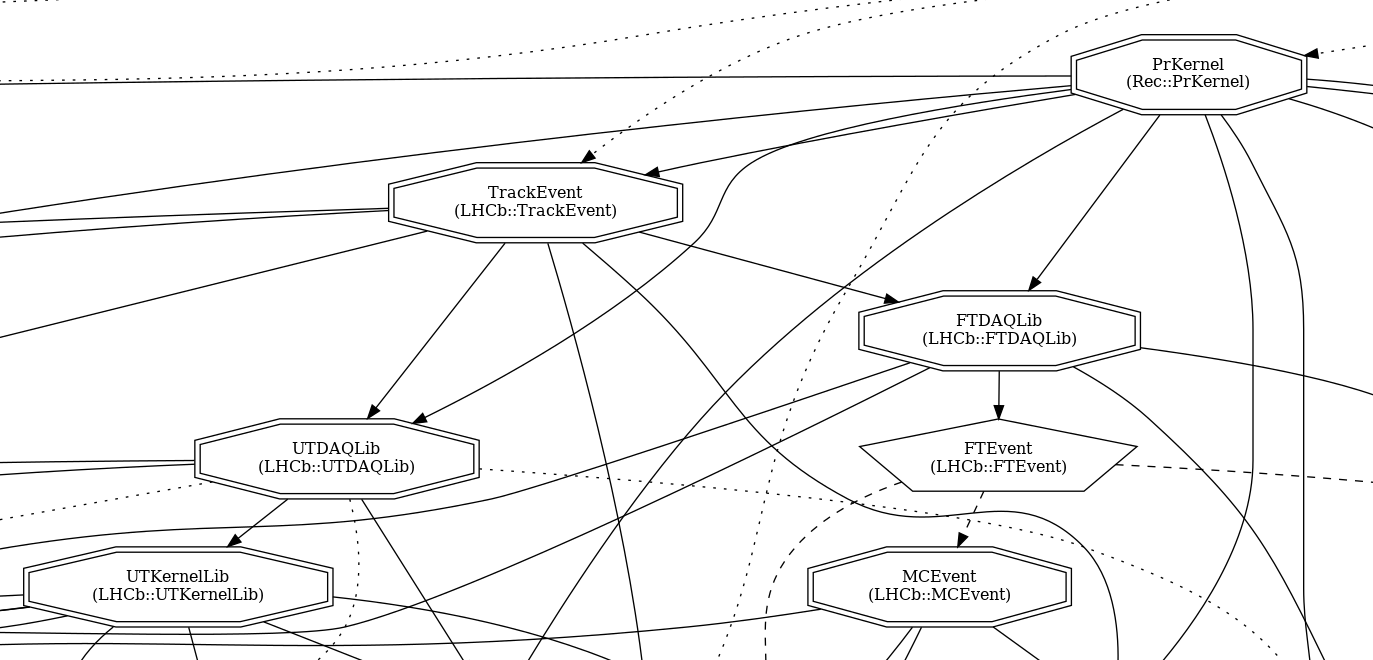
\includegraphics[width=\textwidth]{graphviz_cropped.png}
    \caption{Graphe des dépendances tracé avec graphviz}
    \label{Graphviz}
\end{figure}

\subsection{Passage des bibliothèques partagées en bibliothèques statiques}
Intéressons-nous au remplacement des bibliothèques partagées par des bibliothèques statiques.
L'enjeu est de voir si l'exécution du code est plus rapide.

C'est l'outil CMake qui compile le code, crée les bibliothèques et les link.
Ainsi, dans le programme Gaudi, il y a déjà des fonctions CMake qui permettent de facilement créer des bibliothèques partagées, \verb'gaudi_add_library', et des modules, \verb'gaudi_add_module'.
Il est donc simple de copier la fonction \verb'gaudi_add_library', qui crée une bibliothèque partagée, en une fonction \verb'gaudi_add_static_library'.
Cette fonction utilise la fonction CMake \verb'add_library' dans laquelle il suffit de changer le paramètre \verb'STATIC' en \verb'SHARED'.

Avec cette nouvelle fonction, il est en théorie facile de remplacer les bibliothèques partagée de la pile LHCb en bibliothèques statiques.

\subsubsection{Position-independant code}
Cependant on peut se retrouver dans un cas où une bibliothèque statique est linkée (et donc intégrée) à une bibliothèque dynamique ou à un module.
Or le principe d'une bibliothèque dynamique est d'être chargée dynamiquement, sa position en mémoire n'est pas connue à priori, elle doit donc être compilée en \emph{position-independant code} pour pouvoir fonctionner.
Ce n'est pas le cas d'une bibliothèque statique pour laquelle on sait à la compilation où son code machine sera en mémoire relativement à l'exécutable.
On doit donc rajouter l'option de compilation \verb'-fpic' pour compiler les bibliothèques statiques en position-independant code (on pourra l'enlever lorsque tout sera statique).

\subsection{Passage des modules en bibliothèques statiques}
Gaudi propose également une fonction CMake \verb'gaudi_add_module'.
On peut donc simplement remplacer les appels à cette fonction par l'appel à la fonction précédemment créée \verb'gaudi_add_static_library'.
Il faut également linker ces nouvelles bibliothèques statiques avec l'exécutable.
Pour cela il suffit d'utiliser la fonction CMake \verb'target_link_libraries' sur l'exécutable.

\subsubsection{whole-archive}
Cette approche permet de compiler, en revanche il y a un problème à l'exécution.
En effet par défaut le linker supprime le code qui n'est pas utilisé.

Or dans la pile LHCb, les modules sont des plugins qui sont chargés sur demande par le programme Gaudi.
Celui-ci contient un service qui fournit des algorithmes à d'autres, et qui charge les plugins correspondant si besoin.
Le mécanisme pour rendre ces algorithmes accessibles est de les enregistrer lors du chargement du module via un appel de fonction.
Ainsi lorsqu'un module est chargé, une fonction est exécutée qui enregistre le module auprès de ce service.

En mode statique, cette fonction n'est plus appelée et est donc supprimée.
De ce fait, tout le reste du code du module n'est plus utilisé et est donc également supprimé.

Résoudre ce problème correctement consisterait à revoir en profondeur le système de plugins de LHCb, ce qui semble trop complexe à ce stade.
La solution retenue a été d'utiliser l'option de linkage \verb'-Wl,--whole-archive' qui force le linker à garder l'ensemble du code.

\subsubsection{allow-multiple-definition}
Cependant certains symboles sont inclus plusieurs fois puisque plusieurs bibliothèques utilisent les mêmes et que \verb'whole-archive' oblige le linker à tout inclure.
Cela mène à une erreur que l'on peut désactiver avec l'option \verb'-Wl,--allow-multiple-definition'.

\subsubsection{export-dynamic}
Un dernier problème est que l'on charge toujours dynamiquement quelques modules, notamment des foncteurs.
Or ceux-ci ont besoin des symboles définis dans les bibliothèques désormais statiques et qui ne sont donc plus visibles.
L'option \verb'-Wl,--export-dynamic' résout ce dernier problème en forçant les symboles à être exportés.

\subsubsection{Résumé}
Ainsi, pour remplacer les modules par des bibliothèques statiques, il faut linker avec les options :
\begin{verbatim}
-Wl,--whole-archive -Wl,--allow-multiple-definition -Wl,--export-dynamic
\end{verbatim}

Il n'est normalement pas recommandé d'utiliser ces options car elles ne correspondent pas au comportement usuel du linker et peuvent donc être à l'origine de bugs ou de mauvaises optimisations.
Cependant pour notre étude elles permettent d'obtenir un exécutable presque entièrement statique (quelques bibliothèques ont du être laissées dynamiques et les foncteurs sont par nature dynamiques).
L'ensemble fonctionne comme le montrent les tests d'intégration qui tournent toujours et sont corrects, et permet de mesurer le gain éventuel.

\section{Guided optimization}
\subsection{Méthode de recherche}
La compilation de la pile complète pouvant prendre plus d'une demi-heure, tester le fonctionnement des différentes options serait très long.
Pour être plus efficace dans l'étape de recherche, j'ai donc d'abord testé les options sur un autre programme plus petit.
J'ai choisi d'utiliser le programme de RayTracing que j'ai développé pour mon TIPE.
Il a les avantages :
\begin{enumerate}
    \item d'être suffisamment complexe pour ne pas être optimisé trivialement par le compilateur ;
    \item de reposer sur l'exécution d'un même algorithme des milliers de fois afin d'obtenir un résultat statistique ;
    \item de compiler en une dizaine de secondes.
\end{enumerate}
De cette manière j'ai pu dans un premier temps comprendre les effets des différentes options avant de les appliquer sur la pile LHCb complète.

\subsection{Profile-guided optimization}
\subsubsection{Mise en place}
Le profile-guided optimization est inclus dans gcc et clang.
Il suffit d'utiliser l'option de compilation \verb'-fprofile-generate' qui va permettre de compiler une version du programme avec instrumentation.

Lorsque cette version de l'exécutable est exécutée, le programme génère des fichiers de profils \verb'.gcda'.
Ceux-ci correspondent à des compteurs qui permettent de connaître l'utilisation de chaque fonction et chaque branchement.

Pour compiler le programme final, l'option \verb'-fprofile-use' est utilisée et les profils sont passés au compilateur.
On peut aussi rajouter l'option \verb'-fprofile-correction' pour corriger certains problèmes qui peuvent apparaître avec le \emph{multi-threading}.
En effet les compteurs utilisés pendant l'instrumentation ne sont pas thread-safe, ils peuvent donc être légèrement faussés.

Ces options sont mises de manière globale sur l'ensemble du projet CMake.

\subsubsection{Difficultés}
Le profile-guided optimization n'a d'abord pas donné de résultats probants, la vitesse d'exécution ne changeant ni sur le test Hlt1 ni sur le test Hlt2.

L'outil VTune créé par \emph{Intel} permet de comprendre l'utilisation du processeur par un programme.
On peut notamment voir le taux de mauvaises prédictions de branchement ou le temps que le processeur passe à attendre la mémoire.
Cet outil a d'abord été utilisé pour voir si le PGO avait un impact sur l'utilisation du processeur.
Cependant, que ce soit pour le test Hlt1 (Figure \ref{hlt1_vtune_pipe}) ou le test Hlt2 (Figure \ref{hlt2_vtune_pipe}), les résumés VTune sont les mêmes avec ou sans le profile-guided optimization.

\begin{figure}[H]
    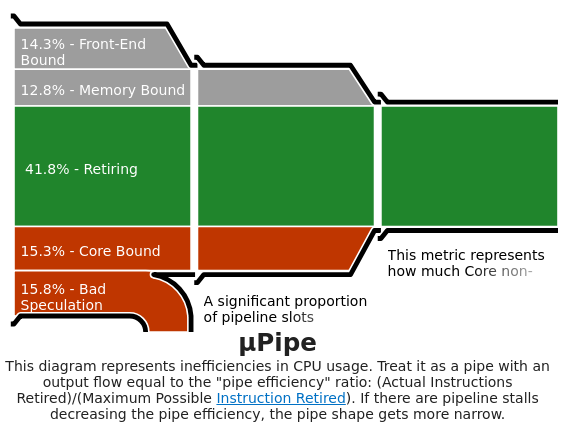
\includegraphics[width=0.8\textwidth, center]{hlt1_vtune_pipe.png}
    \caption{Résumé de VTune pour le test \emph{Hlt1} (référence)}
    \label{hlt1_vtune_pipe}
\end{figure}

\begin{figure}[H]
    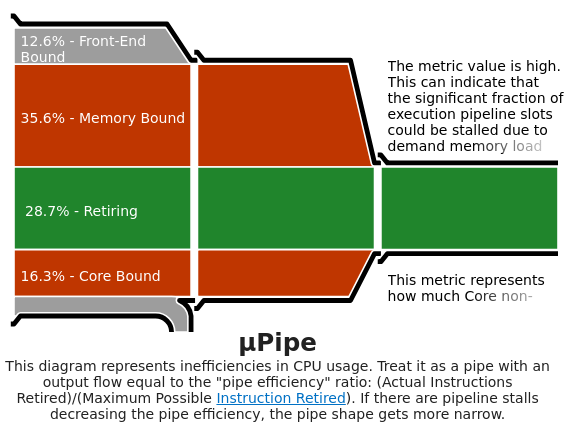
\includegraphics[width=0.8\textwidth, center]{hlt2_vtune_pipe.png}
    \caption{Résumé de VTune pour le test \emph{Hlt2} (référence)}
    \label{hlt2_vtune_pipe}
\end{figure}

Après de plus amples investigations, il est apparu que le PGO n'est efficace que si le link-time optimization est également activé.

\subsection{AutoFDO}
Même si le principe général est similaire, la mise en place d'AutoFDO diffère du PGO.

Tout d'abord la première compilation se fait normalement.

C'est ensuite lorsqu'on exécute le programme qu'on doit le faire en utilisant un outil de profiling.
Le plus simple à utiliser sous Linux est \verb'perf' qui est fourni avec le système.
Cependant ceci nécessite d'avoir certains droits d'administration sur le système.
Une commande typique ressemble à :
\begin{lstlisting}[language=bash]
perf -b -e br_inst_retired.near_taken:pp -- run_command
\end{lstlisting}
Il faut ensuite convertir les fichiers générés au format attendu par le compilateur.
C'est le rôle du programme \verb'create_gcov' fourni par AutoFDO :
\begin{lstlisting}[language=bash]
create_gcov --binary=path/to/binary -- profile=perf.data --gcov=perf.gcov -gcov_version=1
\end{lstlisting}

Enfin l'exécutable est recompilé avec l'option \verb'-fauto-profile=perf.gcov'.

\subsubsection{Difficultés}
Aucune accélération n'a été obtenue avec AutoFDO.
Le PGO a donc été privilégié lorsqu'il a commencé à donner des résultats.
Pour expliquer l'absence d'accélération de l'exécution du programme avec AutoFDO, l'hypothèse la plus probable est que \verb'create_gcov' n'arrive pas à convertir correctement les données issues de \verb'perf'.

\subsection{Link-time optimization}
La mise en place du link-time optimization se fait à deux moments différents :
\begin{enumerate}
    \item tout d'abord au moment de la compilation des fichiers source en fichiers objets,
    \item puis au moment du link.
\end{enumerate}
Avec gcc, cela se fait dans les deux cas via l'option \verb'-flto'.

Cependant CMake supporte nativement le LTO, qui s'appelle ici IPO pour \emph{Interprocedural Optimization}.
Il suffit donc de tester sa disponibilité (lignes 1 et 2) puis de l'activer via une variable dédiée (ligne 3).
\begin{lstlisting}[language=bash,numbers=left]
include(CheckIPOSupported)
check_ipo_supported()
set(CMAKE_INTERPROCEDURAL_OPTIMIZATION TRUE)
\end{lstlisting}
Cette solution a l'avantage de laisser CMake mettre en place le LTO pour la compilation et le link.

On peut remarquer que ceci augmente significativement le temps de link des programmes (environ $50\%$).

\section{Fast-math et stabilité numérique}
\subsection{Comparaison flottante}
\subsubsection{Rappels sur le calcul numérique}
Les nombres flottants étant des approximations, la notion d'égalité stricte perd de son sens.
Deux résultats de calculs sensés être égaux mathématiquement peuvent être différents numériquement.
Cependant l'opérateur de test d'égalité est défini pour les flottants en C et en C++.
Celui-ci vaut vrai si les deux nombres flottants sont strictement identiques, c'est-à-dire si leur représentation est la même bit à bit.
On peut aussi préciser que \verb'-0.0 == +0.0' est vrai tandis que \verb'NaN' n'est égal à rien, pas même à lui-même.
En général, l'utilisation de cet opérateur est dangereuse et doit être évitée.
En effet, les résultats exacts d'un calcul sont dépendant de l'architecture du processeur ou des options de compilation.

Pour repérer ces utilisations, il existe l'option de compilation \verb'-Wfloat-equal' qui imprime un \emph{Warning} pour chaque test d'égalité.
Remplacer ces tests par d'autres tenant compte d'une erreur est important pour éviter qu'un simple arrondi puisse faire basculer les résultats.

\subsubsection{Validité d'une division}
Une utilisation courante du test d'égalité sur les nombres flottants est la division par 0.
Celle-ci étant impossible, il faut trouver un moyen de gérer ce cas en informatique.

On trouve souvent ce genre de code.
\begin{lstlisting}[language=c++,numbers=left]
if (f(x) != 0.)
    return 5./f(x);
else
    ...
\end{lstlisting}
Outre le problème évoqué plus haut concernant la comparaison, on note qu'ici \verb'f(x)' est à priori calculé deux fois et il se pourrait très bien que la première fois son résultat soit proche de 0 sans être égal à 0, tandis que la deuxième fois le résultat soit exactement 0.
Cela peut arriver si par exemple le compilateur décide d'utiliser du \emph{FMA} (jeu d'instructions pour le calcul flottant) pour l'un des deux calculs mais pas l'autre, l'arrondi pouvant être différent.
Ainsi le test de la 1\iere ligne peut passer tout en ayant une division par 0 à la deuxième ligne.

À noter que ce cas précis est déjà apparu en production pour LHCb et a nécessité des heures de débuggage.
En effet, le problème n'a pu être identifié qu'en inspectant le code assembleur généré.

Une solution qui vient à l'esprit serait de ne calculer qu'une seule fois \verb'f(x)'.
\begin{lstlisting}[language=c++,numbers=left]
float y = f(x);
if (y != 0.)
    return 5./y;
else
    ...
\end{lstlisting}
En fait ce code ne résout rien car le compilateur peut encore décider de faire le calcul deux fois (à moins d'utiliser le mot clé \verb'volatile'), si par exemple il estime que c'est plus rapide que de passer par la mémoire.
De plus, même si \verb'f(x)' ne vaut pas 0 mais qu'il en est suffisamment proche, \verb'5./f(x)' peut valoir \verb'+Inf'.

Une solution plus robuste au problème est donc de faire la division puis de vérifier après coup qu'elle s'est bien passée.
Pour cela on peut utiliser \verb'isfinite'.
\begin{lstlisting}[language=c++,numbers=left]
float result = 5./f(x);
if (std::isfinite(result))
    return result;
else
    ...
\end{lstlisting}
Cela à l'avantage de fonctionner peu importe l'opération ou fonction mathématique, et dans le cas d'un enchaînement de calculs on peut faire un seul test sur le résultat final au lieu de tester tous les cas problématiques.

Il est également possible d'utiliser le mécanisme de \emph{trapping} qui permet d'exécuter une interruption par exemple en cas de division par zéro ou de dépassement.
Mais cette méthode se met en place à l'échelle du programme et ne devrait plus être utilisée de nos jours.

\subsection{Fast-math}
On peut activer fast-math en compilant avec l'option \verb'-ffast-math'.
En réalité cette option ne fait qu'en activer d'autres.
Les principales sont :

\subsubsection{no-math-errno}
Cette option permet de ne pas définir la valeur de la variable \verb'errno' après l'appel de fonctions pouvant être exécutées en une instruction (comme \verb'sqrt').
Ce mécanisme de gestion des exceptions ne devrait plus être réellement utilisé en C++ moderne, le désactiver n'est donc pas réellement problématique.

\subsubsection{no-signaling-nans}
Il existe un mécanisme permettant de remonter un signal lorsqu'un calcul est effectué avec une valeur \verb'NaN' comme opérande.
Cette option permet donc de ne pas générer de signal dans un certain nombre de cas.
Celle-ci est activée par défaut.

\subsubsection{no-trapping-math}
Un autre mécanisme génère des interruptions lorsqu'il y a par exemple une division par 0 ou un dépassement (overflow).
Cette option compile en supposant que ces interruptions ne seront pas visibles.

\subsubsection{finite-math-only}
Active des optimisations qui supposent que tous les nombres sont finis (pas de $\pm$Inf ou de NaN).

Ceci peut avoir pour conséquence de remplacer les appels à \verb'isfinite' par \verb'true'.
La plupart des problèmes que l'on peut obtenir à cause de fast-math viennent de cette option pour cette raison.

\subsubsection{no-signed-zeros}
Le compilateur arrête de faire la différence entre $+0.0$ et $-0.0$.
Il peut ainsi simplifier des expressions comme \verb'0.0+x' en \verb'x'.

C'est probablement l'option la plus sûre à activer car peu d'algorithmes nécessitent que $0$ soit signé.

\subsubsection{associative-math}
Les flottants sont désormais considérés comme associatifs.
Cela permet de nombreuses optimisations :
\begin{enumerate}
    \item Simplification d'expressions comme \verb'2.0*x*3.0' en \verb'6.0*x' ;
    \item Simplification de calculs comme \verb'a+b-a' en \verb'b' qui est plus rapide et plus précis.
    \item Meilleure vectorisation des opérations, c'est-à-dire utiliser des instructions du processeur permettant de faire un calcul sur plusieurs données à la fois.
          Par exemple \verb'((a*b)*c)*d' peut être changé en \verb'(a*b)*(c*d)' ce qui permet de calculer \verb'a*b' et \verb'c*d' en même temps.
    \item En réordonnant certains calculs, il est possible d'utiliser des jeux d'instruction du processeur comme le \emph{FMA}.
          Celui-ci permet de faire une multiplication suivie d'une addition en une seule instruction.
\end{enumerate}

Du fait de tous ces changements, les résultats des calculs peuvent changer.
Dans un certain nombre de cas ils peuvent être plus justes du fait du FMA qui est plus précis et des simplifications qui, en réduisant le nombre de calculs, limitent le nombre d'arrondis effectués.
Cependant il existe quelques algorithmes numériques qui reposent sur les règles d'arrondis et qui risquent donc de ne plus fonctionner correctement avec associative-math.

\subsubsection{reciprocal-math}
Pour la plupart des processeurs, il est plus rapide de calculer une multiplication qu'une division.
Ainsi, si on veut diviser plusieurs nombres par un même nombre $y$ (ce qui arrive typiquement lorsqu'on normalise un vecteur), il peut être plus intéressant de calculer une fois l'inverse de $y$ puis de le multiplier à chaque nombre que l'on veut diviser.

C'est ce que permet reciprocal-math qui va remplacer \verb'x/y' par \verb'x*(1/y)' lorsque cela permet un gain de temps.
Ceci peut cependant engendrer une perte de précision.

\subsubsection{unsafe-math-optimizations}
Cette option active no-signed-zeros, no-trapping-math, associative-math, reciprocal-math ainsi que d'autre optimisations comme la non prise en charge des nombres dénormalisés (nombres très proches de $0$).

L'activer change des options du \emph{FPU} ("Floating Point Unit" ou unité de calcul des flottants) du processeur, ce qui peut impacter les autre bibliothèques chargées dynamiquement.
Il y a donc un effet de bord sur les autre bibliothèques qui peut être très difficile à débuguer en cas de problème.

\subsection{Mesure de l'instabilité}
L'objectif premier en activant fast-math est d'accélérer l'exécution du programme.
Mais on remarque qu'en activant certaines de ces options, notamment no-signed-zeros, associative-math et reciprocal-math, on change légèrement la manière de faire certains calculs.
Ainsi, si ces petites différences ont un impact important sur les résultats finaux, cela veut dire que nos algorithmes sont probablement instables numériquement.
Cela peut remettre en cause la validité de certains résultats, il est donc important de les identifier et de les corriger.

L'infrastructure LHCb possède déjà un grand nombre de "compteurs" qui représentent des résultats d'algorithmes.
Ils sont notamment utilisés pour effectuer des tests et permettent donc de repérer si les modifications du code changent leurs valeurs.
Ainsi, il a été possible via un code Python de récupérer ces compteurs et les enregistrer au format \verb'csv'.
On peut ensuite ouvrir ce fichier avec un logiciel de tableur afin de mesurer l'erreur relative entre la référence et la version fast-math et d'en faire des statistiques.

Ainsi on peut voir quels sont les algorithmes les plus sensibles aux options de fast-math et donc probablement numériquement instables.

\section{Include-what-you-use (iwyu)}
\emph{iwyu} a été conçu pour fonctionner avec le compilateur \emph{clang}.
Encore une fois, il est aisé d'utiliser cet outil à travers CMake.
En effet il suffit de donner à la variable \verb'CMAKE_CXX_INCLUDE_WHAT_YOU_USE' la commande \verb'include-what-you-use'.
Il faut alors exécuter CMake avec la version de clang correspondante comme compilateur.

Initialement, une version compatible avec \verb'clang12' a été utilisée car elle était déjà installée sur le système.
Cependant, un bug est apparu : l'outil gère mal certaines références cycliques.
Après recherche, ce bug  est connu mais n'a été corrigé qu'avec la dernière version de iwyu.
Il a donc fallut la télécharger et recompiler avec \verb'clang16', une version plus récente du compilateur.

Cette nouvelle version a permis d'utiliser iwyu mais a mis en lumière un certain nombre de problèmes de l'outil :
\begin{itemize}
    \item suppression d'inclusions pourtant nécessaires ;
    \item ajout d'inclusions pas nécessairement utiles ;
    \item certaines architecture utilisés sont incompatibles avec le principe de l'outil, comme lorsqu'un fichier header définissant des \emph{templates} inclut à sa fin le fichier contenant le code de ces templates (Figure \ref{iwyu_templates}).
\end{itemize}

\begin{figure}[H]
    \begin{center}
        \begin{tikzpicture}[node distance=7cm]
            \tikzstyle{file}=[rectangle,draw,minimum width=6cm,fill=blue!20,text width=6cm]
            \node[file,label={A.hpp}] (hpp) {
                \begin{lstlisting}[language=c++]
#ifndef __A_HPP__
#define __A_HPP__

template<typename T>
class A {
  void function();
};

#include "A.icpp"

#endif
                \end{lstlisting}
            };
            \node[file,right of=hpp,label={A.icpp}] (icpp) {
                \begin{lstlisting}[language=c++]
template<typename T>
void A<T>::function() {
  ...
}
                \end{lstlisting}
            };
            ;
        \end{tikzpicture}
        \caption{Exemple de header déclarant des templates et incluant le fichier contenant leurs définitions}
        \label{iwyu_templates}
    \end{center}
\end{figure}

À cause de ces problèmes, l'idée initiale d'une utilisation systématique d'iwyu a été abandonnée.
L'outil a néanmoins permis de trouver et de corriger des erreurs existantes.

\section{Compilation sur ARM}
La pile LHCb avait déjà été adaptée pour \verb'arm' il y a quelques années.
La plupart des problèmes avaient donc été résolus.
Cependant elle n'a plus été compilée pour cette platforme depuis et le port a donc pu être cassé.
L'enjeu est donc de corriger les nouveaux éventuels problèmes qui sont apparus depuis.

\subsection{Platforme de travail}
Une machine de travail \verb'arm' a été installée pour faire ce travail.
L'architecture précise est \verb'armv8.1_a' et le système d'exploitation est Centos 7.
Le compilateur \verb'gcc11' a de nouveau été utilisé, celui-ci fonctionnant également pour \verb'arm'.

\subsection{MDF}
Dans un premier temps, les programmes Gaudi, Detector et LHCb ont été compilés avec succès.
Cependant à l'exécution, un problème critique est apparu lors de la lecture des fichier \verb'.mdf', un format de fichier spécifique à LHCb.

Le code responsable du parsing de ces fichiers a un fonctionnement particulier.
Il déclare des structures dont la forme correspond au format MDF \cite{edms784588} et s'assure qu'il n'y ait pas de padding (espace mémoire ajouté par le compilateur entre les différents attributs d'une structure afin de les aligner).
Ainsi, lors du parsing d'un fichier, il fait un simple \verb'reinterpret_cast' du pointeur vers les données binaires en un pointeur vers l'une de ces structures.
Bien que fonctionnant, ce code n'est pas standard car si la structure compilée n'a pas exactement la même forme binaire que le format de fichier, les données seront mal interprétées.

Un \verb'hexdump' des données sortie de cet algorithme a été comparé avec un \verb'hexdump' de la référence.
Ceci a permis de remarquer que la seule différence se trouvait au niveau du \verb'checksum'.

Plusieurs algorithmes de \verb'checksum' sont en effet implémentés et il y avait un problème dans l'un d'eux :

\begin{lstlisting}[language=c++,numbers=left]
unsigned int hash32Checksum( const void* ptr, size_t len ) {
    unsigned int hash = 0;
    const char*  k    = (const char*)ptr;
    for ( size_t i = 0; i < len; ++i, ++k ) {
        hash += *k;
        hash += ( hash << 10 );
        hash ^= ( hash >> 6 );
    }
    hash += ( hash << 3 );
    hash ^= ( hash >> 11 );
    hash += ( hash << 15 );
    return hash;
}
\end{lstlisting}

Cette fonction prend en paramètre un pointeur vers des données binaires qui étaient interprétées comme des caractères.
Or en C il n'est pas définit si le type \verb'char' est par défaut signé ou non ; et il se trouve que sur platforme \verb'x86_64' il est signé, alors qu'il ne l'est pas sur \verb'arm'.
Les opérations effectuées sur ces caractères n'étaient donc pas ceux attendus sur \verb'arm'.

La solution a simplement été d'explicitement ajouter \verb'unsigned' devant chaque \verb'char' à la ligne 3 :
\begin{lstlisting}[language=c++]
signed const char*  k    = (const signed char*)ptr;
\end{lstlisting}

Après cette correction, tous les problèmes restant dans le programme LHCb n'étaient que des problèmes mineurs, comme des tests qui vérifiaient la prise en charge de fonctionnalités non disponibles sur \verb'arm'.

\subsection{Catboost}
La compilation du programme Rec a ensuite été tentée.
Le seul problème se situe dans un algorithme nommé \verb'MuonID' qui dépend de \verb'catboost', une bibliothèque externe.
Celle-ci n'est en effet pas disponible sur \verb'arm' pour la release utilisée par LHCb, qui s'avère être relativement ancienne.

Les dernières versions du code de \verb'catboost' peuvent être compilées pour \verb'arm' mais ce n'est pas le cas des plus anciennes.
Une solution serait donc de passer à une version plus récente.

Au problème technique s'ajoute en outre un problème institutionnel.
Catboost est en effet développé par des ingénieurs de l'entreprise russe \emph{Yandex} qui faisait partie de la collaboration LHCb mais qui en a été en partie exclue depuis l'invasion de l'Ukraine par la Russie.
Le support de cette bibliothèque n'est donc plus garantie pour LHCb.
Or comme \verb'MuonID' est le seul algorithme qui l'utilise, la décision de trouver une alternative est donc posée.

En attendant, il a été possible de compiler Rec sans \verb'MuonID'.
Malheuresement, un grand nombre de tests dépendent de cet algorithme pour fonctionner, dont le test Hlt2 utilisé pour les mesures de performances dans le chapitre 3.
En revanche le test Hlt1 qui n'en dépend pas a fonctionné normalement, ce qui montre que la pile LHCb peut au moins en partie fonctionner sur \verb'arm'.


\chapter{Résultats}

\section{Amélioration de la vitesse d'exécution}
Pour mesurer les améliorations, des \emph{throughput tests} ont été menés.
Ceux-ci consistent à exécuter les algorithmes sur 1000 évènements.
On mesure le temps entre $10\%$ et $90\%$ des évènements traités afin de laisser le cache se remplir et de ne mesurer que le temps de calcul (et pas le temps de chargement).
De plus, on exécute le test sur un seul noeud NUMA afin d'éviter de possibles limitations dues à l'architecture NUMA.
On obtient pour chaque test le nombre d'évènements traités par secondes.
Il suffit ensuite de comparer le résultat du test avec celui de la référence qui est fait dans les mêmes conditions pour obtenir l'amélioration.

\emph{Hlt1}, qui fait une reconstruction partielle et rapide, a été testé sur la version statique et PGO, mais aucune amélioration n'a été observée.
Son code ayant déjà été optimisé il y a quelques temps, ce n'est pas étonnant.

Le test \emph{Hlt2}, qui fait une reconstruction complète et plus lente, a lui aussi été testé et a cette fois permis d'obtenir des améliorations.
Celles-ci sont présentées dans les sections suivantes.

\section{Bibliothèques statiques}
Le travail effectué a permis de remplacer les bibliothèques partagées et les modules par des bibliothèques statiques à l'exception de quelques unes.
Ainsi, l'exécutable final passe de $20 Ko$ à $2,5 Go$ et contient pratiquement tout le code de la pile.

Des \emph{throughput tests} ont été effectués :
\begin{figure}[H]
    \begin{center}
        \begin{tabular}{ c c c }
            Optimisation & Amélioration & Intervalle de confiance ($2\sigma$) \\
            Static       & $0.87\%$     & $\pm 0.60\%$
        \end{tabular}
    \end{center}
    \caption{Amélioration de la vitesse d'exécution avec des bibliothèques statiques par rapport à la référence}
    \label{results_static}
\end{figure}

Aucune amélioration significative en ce qui concerne la vitesse d'exécution n'est visible.
Au vue des problèmes rencontrées pour sa mise en oeuvre, cette piste a donc été abandonnée.

\section{Guided optimization}
Le profile-guided optimization a permis pendant les phases de recherche d'obtenir une accélération lorsqu'il était conjointement utilisé avec le link-time optimization.
Cela n'a pas été le cas avec AutoFDO.

\subsection{Code final}
Le code ajouté au CMake global du projet est finalement relativement simple.
Il utilise deux variables :
\begin{itemize}
    \item \verb'PGO' définit le mode de compilation :
          \begin{itemize}
              \item standard si la variable n'est pas définie ;
              \item génération des profils si elle vaut \verb'GENERATE' ;
              \item utilisation des profils si elle vaut \verb'USE'.
          \end{itemize}
    \item \verb'PGO_PATH' est optionnelle et permet de spécifier le dossier où créer et utiliser les profils qui sont par défaut dans les dossiers de build si la variable n'est pas définie.
\end{itemize}

Le mode génération des profils est pris en compte par le code suivant :
\begin{lstlisting}[language=bash,numbers=left]
if("${PGO}" MATCHES "GENERATE")
	message("PGO generate")
        # Ajout du flag -fprofile-generate
	if(DEFINED PGO_PATH)
		set(CMAKE_CXX_FLAGS "${CMAKE_CXX_FLAGS} -fprofile-generate=${PGO_PATH}")
	else()
		set(CMAKE_CXX_FLAGS "${CMAKE_CXX_FLAGS} -fprofile-generate")
	endif()
endif()
\end{lstlisting}

De même le mode utilisation des profils est géré par le code :
\begin{lstlisting}[language=bash,numbers=left]
if("${PGO}" MATCHES "USE")
	message("PGO use")
        # Ajout des flags -fprofile-use et -fprofile-correction
	if(DEFINED PGO_PATH)
		set(CMAKE_CXX_FLAGS "${CMAKE_CXX_FLAGS} -fprofile-use=${PGO_PATH} -fprofile-correction")
	else()
		set(CMAKE_CXX_FLAGS "${CMAKE_CXX_FLAGS} -fprofile-use -fprofile-correction")
	endif()
        # Activation du LTO
	include(CheckIPOSupported)
	check_ipo_supported() # Erreur si LTO non supporte
	set(CMAKE_INTERPROCEDURAL_OPTIMIZATION TRUE)
endif()
\end{lstlisting}
À noter ici les lignes 10 à 12 qui permettent de vérifier le support du LTO et de l'activer le cas échéant.

\subsection{Performances}
Ainsi des \emph{throughput tests} ont été réalisés pour le LTO seul et pour le PGO + LTO.
Une version combinant la version statique avec le PGO et le LTO a également été testée :
\begin{figure}[H]
    \begin{center}
        \begin{tabular}{ c c c }
            Optimisation      & Amélioration & Intervalle de confiance ($2\sigma$) \\
            LTO               & $0.17\%$     & $\pm 1.12\%$                        \\
            LTO \& PGO        & $6.74\%$     & $\pm 1.44\%$                        \\
            Static LTO \& PGO & $6.88\%$     & $\pm 0.83\%$
        \end{tabular}
    \end{center}
    \caption{Amélioration de la vitesse d'exécution avec du profile-guided optimization par rapport à la référence}
    \label{results_pgo}
\end{figure}

Le profile-guided optimization combiné au link-time optimization apporte un net gain de performance (environ $7\%$).
Ceci peut représenter plusieurs centaines de machines à l'échelle des centres de calculs de LHCb.

\subsection{Mise en production}
En l'état actuel de la pile LHCb, il n'est pas évident de mettre en production une version PGO.
En effet les projets sont pour l'instant compilés et installés un à un.
Or le PGO nécessite de tout compiler une première fois pour pouvoir exécuter le programme et créer les profils.
Il faudrait donc faire évoluer la manière d'installer les programmes pour utiliser plus simplement cette version.

Cette évolution est déjà en cours pour d'autres raisons, mais prendra du temps à être mises en place.

\section{Fast-math}
Fast-math regroupe de nombreuses options.
Après quelques tests, il a été décidé de ne pas utiliser finite-math-only car il supprime la possibilité d'utiliser des flottants non-finis, or le code LHCb en dépend à quelques endroits.
De même unsafe-math-optimization a des effets de bords subtiles sur les bibliothèques chargées dynamiquement et n'a donc pas été considéré.
Dans la suite, le terme \emph{fast-math} désigne donc toutes les options fast-math à l'exception des deux précédemment citées.

\subsection{Amélioration des performances}
Les options testées ont donc été associative-math et ses dépendances no-signed-zeros et no-trapping-math ;
ainsi que fast-math (associative-math avec no-math-errno et reciprocal-math en plus).
Fast-math a également été testé conjointement avec avec le LTO et le PGO pour voir si les gains sont cumulatifs.
En effet il se pourrait que les deux optimisations jouent sur le même élément, par exemple le nombre d'accès mémoires, au quel cas les gains de performances pourraient ne pas se cumuler.
\begin{figure}[H]
    \begin{center}
        \begin{tabular}{ c c c }
            Optimisation               & Amélioration & Intervalle de confiance ($2\sigma$) \\
            Fast-math                  & $5.06\%$     & $\pm 0.98\%$                        \\
            Associative-math seulement & $4.73\%$     & $\pm 1.51\%$                        \\
            (LTO \& PGO)               & $6.74\%$     & $\pm 1.44\%$                        \\
            Fast-math + LTO \& PGO     & $11.02\%$    & $\pm 0.98\%$
        \end{tabular}
    \end{center}
    \caption{Amélioration de la vitesse d'exécution avec fast-math par rapport à la référence}
    \label{results_fast-math}
\end{figure}

Fast-math permet un important gain de performance (environ $5\%$ d'amélioration),
gain qui se cumule en grande partie avec celui du PGO ce qui conduit à une amélioration de plus de $10\%$ lorsqu'ils sont associés.

Ce gain vient principalement de l'option associative-math, les autres options n'ont donc pas beaucoup d'effet.
Pour l'expliquer, on peut utiliser VTune pour voir le temps que passe le processeur à faire des calculs flottants.

\begin{figure}[H]
    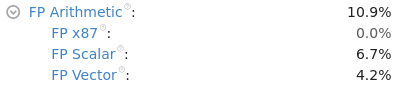
\includegraphics[width=0.75\textwidth, center]{reference_vtune.png}
    \caption{Référence}
    \label{reference_vtune}
\end{figure}

\begin{figure}[H]
    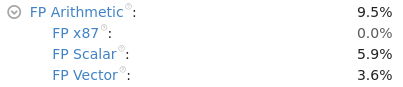
\includegraphics[width=0.75\textwidth, center]{associative-math_vtune.png}
    \caption{Associative-math}
    \label{associative-math_vtune}
\end{figure}

On observe sur les figures \ref{reference_vtune} et \ref{associative-math_vtune} qu'avec associative-math, le processeur réduit d'environ $10\%$ le temps passé dans l'unité de calculs flottants.
De plus, on voit en comparant les figures \ref{hlt2_vtune_pipe} et \ref{fast-math_vtune_pipe} que proportionnellement, le temps passé à attendre le pipeline a diminué mais que celui à attendre la mémoire a augmenté.
Cela peut s'expliquer par le fait qu'en faisant moins de calculs, le processeur est mieux utilisé et que donc la limite de performances se déplace vers la mémoire.

\begin{figure}[H]
    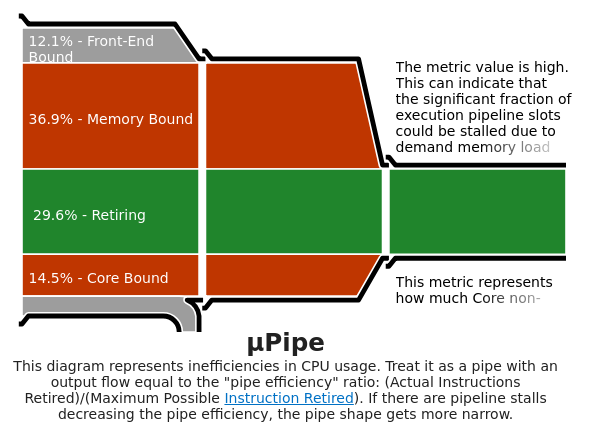
\includegraphics[width=0.8\textwidth, center]{fast-math_vtune_pipe.png}
    \caption{Résumé de VTune pour le test \emph{Hlt2} (fast-math)}
    \label{fast-math_vtune_pipe}
\end{figure}

\subsection{Mesure de l'instabilité}
Le script Python présenté plus haut permet de récupérer la totalité des compteurs utilisés dans la pile LHCb (un peu plus de 30 000).
Ces compteurs sont principalement de deux sortes :
\begin{itemize}
    \item des entiers, qui comptent par exemple le nombre de particules d'un type détectées.
    \item un triplé d'un entier et de deux flottants représentants le nombre d'éléments, la somme et la moyenne d'une valeur.
          Ce type de compteur peut par exemple être utilisé pour représenter l'énergie des particules.
\end{itemize}
Certains de ces compteurs représentent des valeurs directement intéressantes (comme le résultat d'un algorithme) ;
d'autres des valeurs intermédiaires comme la différence ($\chi^2$) d'un algorithme numérique.
Ces derniers sont très sensibles et fluctuent donc beaucoup plus.

Toutes ces données ont été chargées dans le logiciel LibreOffice Calc.
Pour chaque compteur, les erreurs absolues et relatives avec la référence ont été calculées et ont ensuite été triés en fonction de l'erreur relative croissante.

\begin{figure}[H]
    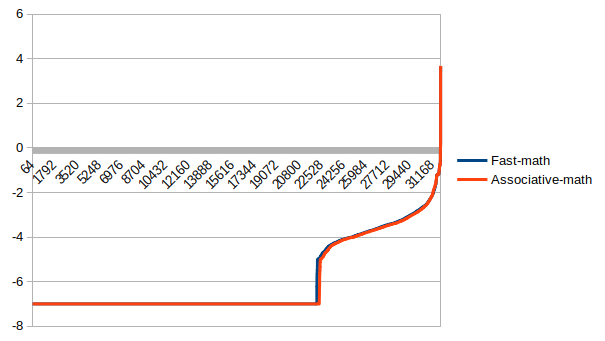
\includegraphics[width=\textwidth, center]{fast-math_difference.png}
    \caption{Logarithme de l'erreur relative des compteurs entre la référence et les versions fast-math et associative-math}
    \label{fast-math_difference}
\end{figure}

Le graphe de la figure \ref{fast-math_difference} représente la distribution de ces erreurs.
L'abscisse donne le nombre de compteurs en dessous d'une erreur relative donnée.
En ordonnée est représenté le logarithme en base 10 de l'erreur relative.
Si l'erreur est nulle, la valeur $-7$ est utilisée car c'est à peu près la précision des flottants 32 bits.

Le graphe montre qu'un certain nombre de compteurs ont une différence significative avec la référence.
Une erreur relative plus grande que $10^{-4}$ ou $10^{-3}$ est trop importante pour la physique.
C'est ici le cas pour plusieurs milliers de compteurs.
Un ou plusieurs algorithmes sont donc probablement trop instables numériquement et devraient être corrigés.

Les graphes de la version associative-math et de la version fast-math ont des courbes quasiment identiques.
Ainsi c'est bien le changement d'ordre des opérations mathématiques qui a un impact sur les résultats numériques.

Ce travail a permis de contacter les auteurs des algorithmes qui divergent le plus pour initier une réflexion sur leur stabilité.

\chapter*{Réflexions sur la responsabilité sociétale et environnementale}
\section*{Enjeux sociétaux}
Le CERN est une organisation internationale dont le but premier est la recherche, il n'est pas à but lucratif.
Si les états membres investissent des milliards c'est parce qu'il est probable que dans plusieurs décennies, les découvertes qui y sont faites auront un grand impact sur nos sociétés,
comme a pu l'être la physique quantique qui a par exemple permis l'informatique ou toutes les technologies utilisant des lasers.
Le Web, qui a été développé afin de plus facilement partager les articles scientifiques est également un bon exemple de technologie ayant marqué le 21\ieme siècle et issue du CERN.

En plus des enjeux liés à la recherche, le CERN a trois autres missions : l'innovation, l'éducation et le rapprochement des nations.
Dans cette perspective, il collabore au sein de plusieurs projets. On peut citer :
\begin{itemize}
    \item \href{https://home.cern/tags/unosat}{UNOSAT}, un projet satellitaire soutenu par les Nations Unies qui permet d'obtenir des renseignements pour l'aide humanitaire. Le CERN fournit toute l'infrastructure informatique du projet ;
    \item \href{https://enlight.web.cern.ch/}{ENLIGHT} qui vise le développement de l'hadronthérapie, méthode permettant de faire de la radiothérapie de manière plus localisée ;
    \item \href{https://home.cern/tags/sesame}{SESAME} pour le développement de la recherche en physique des particules au Moyen-Orient et qui fait travailler ensemble des chercheurs israéliens et palestiniens au sein du même projet.
\end{itemize}

\section*{Enjeux environnementaux}
Le CERN utilise un grand nombre d'installations très gourmandes en énergie qui peuvent donc avoir un impact sur l'environnement.
La consommation électrique du complexe d'accélérateurs peut atteindre $200MW$, ce qui pour comparaison représente un tiers de la consommation de la ville de Genève.
Cette électricité provient principalement de France et est donc en grande partie décarbonée.
Le CERN tente de limiter sa consommation via différents moyens, notamment avec une utilisation plus importante des supraconducteurs au LHC ou la récupération de chaleur dans le nouveau centre de calculs.
Les efforts en matière d'économies d'énergie ont permis au CERN d'être certifié ISO 50001.

En optimisant l'exécution des programmes de LHCb, ce stage a participé à une politique de sobriété qui cherche à mieux utiliser les ressources disponibles au lieu d'en utiliser de nouvelles.


\chapter*{Conclusion}
L'objectif de ce stage était de proposer et d'implémenter des solutions pour accélérer les programmes de reconstruction et d'analyse de LHCb via des optimisations à la compilation.
Plusieurs résultats ont donc été obtenus :
\begin{itemize}
    \item Utiliser des bibliothèques statiques au lieu de bibliothèques dynamiques ne semble pas apporter de gains substantiels et soulève plusieurs problèmes.
          Il ne semble donc pas intéressant de mettre en place cette solution.
    \item Le profile-guided optimization apporte en revanche une accélération significative de l'ordre de $7\%$.
          Il serait donc intéressant de le mettre en place pour l'environnement de production.
    \item Certaines des optimisations regroupées sous la dénomination fast-math permettent également des gains importants de l'ordre de $5\%$.

          Les flags \verb'-fno-trapping-math -fno-signed-zeros -fassociative-math' seraient intéressant à activer,
          \begin{itemize}
              \item dans un premier temps afin de pouvoir suivre l'instabilité numérique,
              \item dans un second temps pour utiliser fast-math en production, en complément du PGO pour obtenir le gain de performance maximal.
          \end{itemize}
\end{itemize}

Ces optimisations indépendantes permettraient d'atteindre en cumulé plus de $10\%$ d'accélération pour les machines de productions.

Enfin, ce stage a permis d'apporter des corrections à la base de code dont certaines permettent désormais de faire tourner la pile LHCb sur architecture \verb'arm'.

\printbibliography
\pagenumbering{gobble}

\end{document}
